\chapter{Dynamical Characterization of Reservoir States for Interpretable Affective Response Analysis}
\label{chap:dynamics}

\section{Introduction and Motivation}

The question is whether the reservoir's internal dynamics carry signatures of the input's temporal organization that are distinct from the information captured by the embedding---whether, in other words, the driven nonlinear system encodes a separate form of hidden order in its trajectory properties. This chapter is the interpretability core of the dissertation: it is where the reservoir ceases to be a feature generator and becomes a \emph{measurement instrument} that produces named, physically grounded descriptors of the input signal.

The preceding chapters established ARSPI-Net as a hybrid architecture in which a Liquid State Machine (LSM) performs temporal state expansion and a graph neural back end performs relational inference across channels. Up to this point, the dissertation has asked a discriminative question: can the transformed representation support accurate inference? That question is necessary, but it does not address the interpretability requirement on $\phi$ established in Chapter~\ref{chap:introduction} (Section~\ref{sec:inverse_problem}): the internal variables of the mapping must be meaningful to both engineers and clinicians. A classification output---however accurate---is opaque. A dynamical descriptor with a name, a unit, and a direct mapping to the input ERP is interpretable.

This chapter addresses that requirement directly. It develops a dynamical characterization framework for the validated reservoir operating point ($\beta = 0.05$, $M_{th}=0.5$, $N_{res}=256$), extracts seven named state-space descriptors from reservoir activity driven by all $633$ observations in the SHAPE dataset, and tests whether these descriptors vary with emotional condition and clinical status. The three metric families---sparse coding efficiency, driven trajectory complexity, and relaxation-time behavior---convert the reservoir from a useful but opaque feature generator into an analyzable nonlinear measurement instrument whose outputs a clinician can inspect without post-hoc explanation methods.

The experimental results (Section~\ref{sec:ch6_results}) reveal a clean dissociation: all seven dynamical metrics are condition-sensitive (Friedman $p < 0.05$ for every metric), with the temporal-structure family ($\hat{H}_{\pi}$, $\tau_{AC}$) carrying $2.4\times$ larger condition effects than the amplitude-tracking family. The dynamical metrics are not clinically sensitive at the channel-averaged level (zero of $49$ metric-diagnosis comparisons reach significance), though the layer ablation in Chapter~\ref{chap:arspi_net} demonstrates that per-channel dynamical features carry the strongest SUD and PTSD clinical signals in the ablation matrix. This dissociation identifies the dynamical response as a distinct information layer within ARSPI-Net---one that encodes what stimulus is being processed rather than whose brain is processing it. The seven descriptors organize subjects along a continuous excitability--persistence axis (Section~\ref{sec:ch6_latent_axis}) that is condition-modulated but not reducible to psychiatric diagnosis---providing clinicians with a one-dimensional characterization of each patient's reservoir response organization.

\section{Notation and Formal Definitions}
\label{sec:dynamics_notation}

We establish notation consistent with Chapters 3--5 and introduce the symbols required for dynamical analysis.

\subsection{The LSM as a Driven Dynamical System}

Let the validated LSM reservoir consist of $N_{res}=256$ leaky integrate-and-fire neurons with fixed random input weights $\mathbf{W}^{in} \in \mathbb{R}^{N_{res} \times N_f}$, fixed random recurrent weights $\mathbf{W}^{rec} \in \mathbb{R}^{N_{res} \times N_{res}}$, membrane decay parameter $\beta=0.05$ (corresponding to $\tau_m \approx 20$ time steps), and firing threshold $M_{th}=0.5$. The reservoir receives a single-channel EEG epoch as its driving input.

\paragraph{Definition 6.1 (Input Process).}
For a given subject $s$ and trial $j$, let $\mathbf{u}^{(j)}_s(t) \in \mathbb{R}^{N_f}$ denote the preprocessed EEG input vector at discrete time step $t \in \{1,\ldots,T\}$, where $T$ is the epoch length and $N_f$ is the number of input features per time step.

\paragraph{Definition 6.2 (Reservoir State).}
The complete reservoir state at time $t$ is the membrane potential vector
\begin{equation}
\mathbf{M}(t) = [M_1(t), M_2(t), \ldots, M_{N_{res}}(t)]^{\top} \in \mathbb{R}^{N_{res}}
\end{equation}
with discrete-time LIF dynamics
\begin{equation}
M_i[t] = (1-\beta)M_i[t-1](1-S_i[t-1]) + I_{tot,i}[t]
\end{equation}
where $S_i[t-1] \in \{0,1\}$ is the spike indicator at the previous step and
\begin{equation}
I_{tot,i}[t] = \sum_{j=1}^{N_f} W^{in}_{ij}u_j(t) + \sum_{\ell=1}^{N_{res}} W^{rec}_{i\ell}S_{\ell}[t-1].
\end{equation}
A spike is emitted when $M_i[t] \ge M_{th}$:
\begin{equation}
S_i[t] = \Theta(M_i[t]-M_{th})
\end{equation}
where $\Theta(\cdot)$ is the Heaviside step function.

\paragraph{Definition 6.3 (Spike Train Matrix).}
For a given trial, the complete spike output of the reservoir is the binary matrix
\begin{equation}
\mathbf{S} \in \{0,1\}^{N_{res}\times T}, \qquad S_{i,t}=S_i[t].
\end{equation}

\paragraph{Definition 6.4 (Global Firing Rate).}
The instantaneous population firing rate at time $t$ is
\begin{equation}
r(t)=\frac{1}{N_{res}}\sum_{i=1}^{N_{res}} S_i[t].
\end{equation}

\paragraph{Definition 6.5 (Driven System Emphasis).}
For a fixed reservoir instantiation (fixed $\mathbf{W}^{in}$ and $\mathbf{W}^{rec}$), the reservoir state trajectory $\mathbf{M}(1),\mathbf{M}(2),\ldots,\mathbf{M}(T)$ is a deterministic function of the input sequence $\mathbf{u}(1),\mathbf{u}(2),\ldots,\mathbf{u}(T)$. We denote the mapping from input sequence to state trajectory as
\begin{equation}
\mathcal{R}: \mathbb{R}^{N_f \times T} \rightarrow \mathbb{R}^{N_{res} \times T}.
\end{equation}
All dynamical metrics extracted in this chapter are properties of $\mathcal{R}(\mathbf{u})$, the driven trajectory, not of $\mathcal{R}$ in isolation.

\section{Metric I: Sparse Coding Efficiency ($\Phi$)}
\label{sec:dynamics_phi}

\subsection{Theoretical Foundation}

The efficient coding hypothesis posits that neural systems evolve or adapt to maximize information transmission while minimizing metabolic expenditure \cite{barlow_possible_1961,olshausen_emergence_1996}. In neuromorphic computing, this principle becomes an energy--information trade-off: the number of joules, or equivalently synaptic operations, expended per bit of transmitted information. In the context of ARSPI-Net, the working hypothesis is that affective dysregulation will manifest as a measurable departure from efficient spike-based coding in the reservoir's response to emotionally salient stimuli. Specifically, pathological inputs may drive the reservoir into a regime of denser, metabolically wasteful firing that carries less stimulus-specific information per spike.

\subsection{Formal Metric Definition}

\paragraph{Definition 6.6 (Total Synaptic Operations).}
For a single trial with spike train matrix $\mathbf{S}$, the total synaptic operations count is
\begin{equation}
\mathrm{SynOps} = \sum_{t=1}^{T} \left[ \sum_{i=1}^{N_{res}} S_i[t] \cdot \left(\mathrm{fan\mbox{-}out}^{rec}_i + \mathrm{fan\mbox{-}out}^{read}_i\right) \right]
\end{equation}
where $\mathrm{fan\mbox{-}out}^{rec}_i$ is the number of nonzero outgoing recurrent connections from neuron $i$ and $\mathrm{fan\mbox{-}out}^{read}_i$ is the number of readout connections. For a fully connected readout to $N_{out}$ output neurons,
\begin{equation}
\mathrm{SynOps} = \sum_{t=1}^{T} \sum_{i=1}^{N_{res}} S_i[t] \cdot (d_i^{rec}+N_{out})
\end{equation}
where $d_i^{rec}$ is the recurrent out-degree of neuron $i$.

Under sparse random connectivity with connection probability $p_c$, the expected recurrent fan-out per neuron is $p_cN_{res}$, yielding the simplified estimator
\begin{equation}
\mathrm{SynOps} \approx N_{total\_spikes}\cdot (p_cN_{res}+N_{out})
\end{equation}
where $N_{total\_spikes}=\sum_{i,t} S_{i,t}$ is the total spike count over the epoch.

\paragraph{Definition 6.7 (Neuromorphic Energy Cost).}
Using a standard neuromorphic hardware energy model in which each synaptic operation costs $E_{syn}$, the trial-level energy cost is
\begin{equation}
E_{trial}=\mathrm{SynOps}\cdot E_{syn}. 
\end{equation}

\paragraph{Definition 6.8 (Spike-Based Mutual Information Estimator).}
To quantify the information content of the reservoir spike response about the stimulus class $y\in\{c_1,c_2,\ldots,c_K\}$, let $f(\mathbf{S})$ denote the feature vector extracted from the spike train, for example the $\mathrm{BSC}_6 \rightarrow \mathrm{PCA}\text{-}64$ embedding validated in Chapter 4. The decoded mutual information is bounded below by the Fano-type estimator
\begin{equation}
I_{decoded}(\mathbf{S};y) \ge \log_2(K) - H_b(P_e)
\end{equation}
where $P_e$ is the Bayes-optimal classification error rate estimated via cross-validation and $H_b(\cdot)$ is the binary entropy function. A refined estimate can be obtained from the normalized confusion matrix:
\begin{equation}
\hat{I}(\mathbf{S};y)=\sum_{k=1}^{K}\sum_{\hat{k}=1}^{K} p(y=k,\hat{y}=\hat{k})\log_2\!\left(\frac{p(y=k,\hat{y}=\hat{k})}{p(y=k)\,p(\hat{y}=\hat{k})}\right).
\end{equation}

\paragraph{Definition 6.9 (Sparse Coding Efficiency).}
The sparse coding efficiency metric is
\begin{equation}
\Phi = \frac{\hat{I}(\mathbf{S};y)}{\mathrm{SynOps}} \qquad \left[\frac{\mathrm{bits}}{\mathrm{synaptic\ operation}}\right]
\end{equation}
or, in physical units,
\begin{equation}
\Phi_E = \frac{\hat{I}(\mathbf{S};y)}{E_{trial}} \qquad \left[\frac{\mathrm{bits}}{\mathrm{Joule}}\right].
\end{equation}

\subsection{Auxiliary Metrics}

\paragraph{Definition 6.10 (Population Sparsity).}
The lifetime sparsity of the population response is measured by the Treves--Rolls sparsity index
\begin{equation}
a = \frac{\left(\frac{1}{N_{res}}\sum_{i=1}^{N_{res}} \bar{r}_i\right)^2}{\frac{1}{N_{res}}\sum_{i=1}^{N_{res}} \bar{r}_i^2}
\end{equation}
where $\bar{r}_i=(1/T)\sum_t S_i[t]$ is the mean firing rate of neuron $i$ over the epoch.

\paragraph{Definition 6.11 (Temporal Sparsity).}
The fraction of time steps in which the population is quiescent is
\begin{equation}
a_{temp}=\frac{1}{T}\sum_{t=1}^{T} \mathbb{1}[r(t)<\epsilon].
\end{equation}
In implementation, $\epsilon$ may be chosen as $1/N_{res}$, corresponding to at most one spike per time step.

\subsection{Hypothesis H1}
The efficient coding hypothesis predicts that for subjects in the healthy control (HC) group, the reservoir response to negative-valence stimuli will exhibit higher $\Phi$ than the response generated by subjects in the Major Depressive Disorder (MDD) group:
\begin{equation}
\mathbb{E}[\Phi\mid \mathrm{HC}] > \mathbb{E}[\Phi\mid \mathrm{MDD}].
\end{equation}
This hypothesis is tested in Section~\ref{sec:ch6_results}, EXP-6.6.

\section{Metric II: Driven Trajectory Complexity ($\Lambda$)}
\label{sec:dynamics_lambda}

\subsection{Theoretical Foundation}

The edge-of-chaos hypothesis for reservoir computing posits that recurrent networks have maximal computational capacity near a dynamical phase transition between strongly contracting and strongly expanding dynamics \cite{langton_computation_1990,bertschinger_real-time_2004}. In driven systems, the relevant quantity is not the autonomous Lyapunov spectrum of the reservoir in isolation, but the conditional or driven Lyapunov exponent: the exponential separation rate of nearby trajectories under the \emph{same} input drive. The affective-processing interpretation considered here is that healthy dynamics preserve a richer, more flexible temporal repertoire, whereas pathological dynamics collapse toward a lower-dimensional and more repetitive response manifold.

\subsection{Formal Metric Definitions}

\subsubsection{The Largest Lyapunov Exponent of the Driven Reservoir}

\paragraph{Definition 6.12 (Driven Lyapunov Exponent).}
Consider the driven reservoir as a discrete-time dynamical system
\begin{equation}
\mathbf{M}[t+1]=\mathbf{F}(\mathbf{M}[t],\mathbf{u}[t]).
\end{equation}
The driven Lyapunov exponent quantifies the average exponential rate of separation of infinitesimally close trajectories under the same input drive. Let $\delta \mathbf{M}[0]$ be a small perturbation to the initial state and let the perturbed trajectory evolve as
\begin{equation}
\mathbf{M}'[t+1]=\mathbf{F}(\mathbf{M}'[t],\mathbf{u}[t]).
\end{equation}
Then
\begin{equation}
\lambda_1 = \lim_{T\to\infty}\frac{1}{T}\sum_{t=0}^{T-1}\ln\frac{\lVert \delta \mathbf{M}[t+1]\rVert}{\lVert \delta \mathbf{M}[t]\rVert}
\end{equation}
where $\delta \mathbf{M}[t]=\mathbf{M}'[t]-\mathbf{M}[t]$.

The threshold-and-reset operation in leaky integrate-and-fire dynamics introduces a discontinuity, so the tangent-space calculation must account for spike events explicitly. Event-based Lyapunov calculations for LIF networks have been developed in prior work on spiking-network stability and can be used to motivate the projection treatment at threshold crossings \cite{monteforte_dynamic_2012}. For finite EEG epochs, the practical estimate used in this chapter follows the standard renormalization strategy associated with Benettin-style Lyapunov computation \cite{benettin_lyapunov_1980}:
\begin{enumerate}
    \item Initialize the reservoir at state $\mathbf{M}[0]$ and a nearby state $\mathbf{M}'[0]=\mathbf{M}[0]+\delta_0\hat{\mathbf{e}}$, where $\hat{\mathbf{e}}$ is a random unit vector and $\delta_0=10^{-8}$.
    \item Evolve both trajectories under the same input $\mathbf{u}(t)$ for $T_{renorm}$ steps.
    \item Compute the stretching factor $\gamma_k = \lVert \mathbf{M}'[kT_{renorm}] - \mathbf{M}[kT_{renorm}] \rVert/\delta_0$.
    \item Renormalize the perturbed trajectory along the instantaneous separation direction.
    \item Repeat for $K$ renormalization intervals and estimate
    \begin{equation}
    \hat{\lambda}_1 = \frac{1}{KT_{renorm}}\sum_{k=1}^{K}\ln(\gamma_k).
    \end{equation}
\end{enumerate}

\subsubsection{Lempel--Ziv Complexity ($C_{LZ}$)}

\paragraph{Definition 6.13 (Lempel--Ziv Complexity of Reservoir Spike Output).}
For a single neuron $i$, let $s_i=S_i[1]S_i[2]\cdots S_i[T]$ be the binary spike sequence. The normalized Lempel--Ziv complexity is
\begin{equation}
C_{LZ,i}=\frac{c(s_i)}{T/\log_2(T)}
\end{equation}
where $c(s_i)$ is the number of distinct substrings generated by the LZ76 parsing procedure. The population-level complexity is
\begin{equation}
C_{LZ}=\frac{1}{N_{res}}\sum_{i=1}^{N_{res}} C_{LZ,i}.
\end{equation}

\subsubsection{Permutation Entropy ($H_{\pi}$)}

\paragraph{Definition 6.14 (Permutation Entropy of Membrane Potential Trajectory).}
As a complementary complexity measure operating on the continuous-valued membrane potentials rather than the binary spike trains, define the global mean membrane potential
\begin{equation}
\bar{M}(t)=\frac{1}{N_{res}}\sum_{i=1}^{N_{res}} M_i[t].
\end{equation}
For embedding dimension $d$ and delay $\tau$, ordinal patterns are constructed from $[\bar{M}(t),\bar{M}(t+\tau),\ldots,\bar{M}(t+(d-1)\tau)]$. The permutation entropy is then
\begin{equation}
H_{\pi}=-\sum_{\pi\in S_d} p(\pi)\log_2 p(\pi)
\end{equation}
with normalized form
\begin{equation}
\hat{H}_{\pi}=\frac{H_{\pi}}{\log_2(d!)}.
\end{equation}
Permutation entropy was introduced by Bandt and Pompe as a natural complexity measure for time series \cite{bandt_permutation_2002}.

\subsection{Phase-Space Visualization}

\paragraph{Definition 6.15 (Reconstructed Phase Portrait).}
For visualization and qualitative assessment of attractor geometry, let $\mathbf{M} \in \mathbb{R}^{N_{res}\times T}$ be the membrane potential matrix for a given trial. Compute the PCA projection
\begin{equation}
\mathbf{z}(t)=\mathbf{W}_{PC}^{\top}(\mathbf{M}(t)-\bar{\mathbf{M}}) \in \mathbb{R}^{2}
\end{equation}
where $\mathbf{W}_{PC}=[\mathbf{w}_1,\mathbf{w}_2]$ contains the first two principal-component directions and $\bar{\mathbf{M}}$ is the temporal mean.

\subsection{Hypothesis H2}
The edge-of-chaos hypothesis predicts that reservoir trajectories driven by EEG from healthy control subjects processing negative-valence stimuli will exhibit greater driven complexity than trajectories driven by EEG from MDD subjects:
\begin{equation}
\mathbb{E}[\Lambda\mid \mathrm{HC}] > \mathbb{E}[\Lambda\mid \mathrm{MDD}]
\end{equation}
where $\Lambda \in \{\lambda_1,C_{LZ},\hat{H}_{\pi}\}$. This hypothesis is tested in Section~\ref{sec:ch6_results}, EXP-6.6.

\section{Metric III: Relaxation Time Constant ($T$)}
\label{sec:dynamics_tau}

\subsection{Theoretical Foundation}

Critical slowing down is a phenomenon in nonlinear dynamical systems whereby recovery from perturbations becomes slower as the system approaches a tipping point or loss of stability \cite{scheffer_early-warning_2009}. In psychiatry and affective-dynamics work, elevated temporal autocorrelation has been proposed as an early-warning indicator for depressive transitions \cite{vandeleemput_critical_2014,wichers_critical_2016}. In the reservoir-computing context considered here, the relaxation time quantifies how rapidly the network's activity returns to baseline after an affective stimulus has driven the system away from its resting regime.

\subsection{Formal Metric Definitions}

\subsubsection{Exponential Relaxation Time ($\tau_{relax}$)}

\paragraph{Definition 6.16 (Relaxation Time Constant).}
Consider the global firing rate $r(t)$ during the post-stimulus window $[t_{onset},t_{end}]$. Define
\begin{equation}
r_{peak}=\max_{t\in[t_{onset},t_{end}]} r(t), \qquad t_{peak}=\arg\max_{t\in[t_{onset},t_{end}]} r(t).
\end{equation}
The relaxation phase is $[t_{peak},t_{end}]$. Model the decay of the firing-rate envelope as
\begin{equation}
r(t) \approx r_{\infty} + (r_{peak}-r_{\infty})\exp\left(-\frac{t-t_{peak}}{\tau_{relax}}\right), \qquad t\ge t_{peak}
\end{equation}
where $r_{\infty}$ is estimated from the final portion of the epoch.

\subsubsection{Autocorrelation Decay Rate}

\paragraph{Definition 6.17 (Lag-$k$ Autocorrelation of Population Firing Rate).}
The normalized autocorrelation function of the global firing rate is
\begin{equation}
\rho(k)=\frac{\sum_{t=1}^{T-k}(r(t)-\bar{r})(r(t+k)-\bar{r})}{\sum_{t=1}^{T}(r(t)-\bar{r})^2}
\end{equation}
where $\bar{r}=(1/T)\sum_t r(t)$.

\paragraph{Definition 6.18 (Autocorrelation Decay Constant).}
Define
\begin{equation}
\tau_{AC}=\min\{k\ge 1: \rho(k)\le e^{-1}\}
\end{equation}
or estimate $\tau_{AC}$ by fitting an exponential decay model to $\rho(k)$.

\subsubsection{Attractor Depth via Return-to-Baseline Time}

\paragraph{Definition 6.19 (Return-to-Baseline Time).}
Let the baseline firing rate be
\begin{equation}
r_{baseline}=\frac{1}{|[1,t_{onset}]|}\sum_{t=1}^{t_{onset}} r(t).
\end{equation}
The return-to-baseline time is
\begin{equation}
T_{RTB}=\min\left\{t>t_{peak}: r(t')\le r_{baseline}+\alpha(r_{peak}-r_{baseline})\ \forall\ t'\in[t,t+\Delta]\right\}-t_{peak}
\end{equation}
where $\alpha\in(0,1)$ is a threshold fraction and $\Delta$ is a sustain window.

\subsection{Energy Landscape Interpretation}

The relaxation time can be interpreted through an energy-landscape metaphor from attractor-network theory. Near a locally stable operating point of the autonomous reservoir, the linearized Jacobian determines the slowest decay mode. If $\mu_{max}$ is the eigenvalue of largest magnitude inside the unit disk, then
\begin{equation}
\tau_{relax}^{(slow)} = -\frac{1}{\ln|\mu_{max}|}.
\end{equation}
As $|\mu_{max}|\rightarrow 1^{-}$, the relaxation time diverges, which is the hallmark of critical slowing down.

\subsection{Hypothesis H3}
The critical slowing down literature predicts that reservoir responses to negative-valence stimuli driven by MDD subjects' EEG will exhibit longer relaxation times than those driven by healthy controls:
\begin{equation}
\mathbb{E}[\tau_{relax}\mid \mathrm{MDD}] > \mathbb{E}[\tau_{relax}\mid \mathrm{HC}].
\end{equation}
This hypothesis is tested in Section~\ref{sec:ch6_results}, EXP-6.6.

\section{The Reservoir--Input Mapping Problem}
\label{sec:dynamics_fidelity}

\subsection{The Central Question for Defense}

This section addresses the foundational validity question for the entire dynamical characterization framework: under what formal conditions do dynamical metrics extracted from a driven LSM reservoir constitute valid estimators of properties of the source EEG signal, and by extension, of the cortical dynamics that generated it? This is not a peripheral methodological detail. It is the load-bearing theoretical structure on which any clinical or physiological interpretation of Sections~\ref{sec:dynamics_phi}--\ref{sec:dynamics_tau} depends.

The argument is organized in five layers:
\begin{enumerate}
    \item a measurement-instrument paradigm that clarifies what the reservoir is and is not being claimed to measure;
    \item echo-state and generalized-synchronization arguments establishing initial-condition independence and input determinism;
    \item information-theoretic bounds clarifying what can and cannot be preserved through the reservoir transformation;
    \item Takens-type embedding arguments that motivate dynamical sufficiency under explicit assumptions; and
    \item metric-specific monotonicity and validation arguments.
\end{enumerate}

\subsection{Measurement-Instrument Paradigm}

A spectrum analyzer, oscilloscope, or matched-filter bank has its own internal dynamics, yet one can still use it to characterize an input signal so long as the transformation is calibrated and stable. The reservoir plays an analogous role here. It is a fixed nonlinear dynamical operator whose driven internal trajectory encodes information about the input in a high-dimensional state. The key epistemological point is therefore the following: the dynamical metrics computed in this chapter are not claimed to be identical to latent cortical invariants. They are claims about calibrated functionals of the \emph{driven reservoir response}.

In particular, the dissertation does not claim that the reservoir relaxation time is literally the relaxation time of the cortex. Rather, the claim is that the reservoir relaxation time, when extracted under conditions that guarantee input determinism and adequate fidelity, can serve as a consistent and discriminative functional of the EEG drive. This measurement-instrument framing is central because it prevents a category error that would otherwise weaken the chapter's integrity. The uploaded expansion makes this distinction explicit and correctly treats the reservoir as a standardized nonlinear instrument rather than as a direct physiological surrogate.

\subsection{Formal Signal-Chain Setup}

Let $\theta \in \Theta$ denote a latent clinical or affective state parameter, let $\mathbf{X}(t;\theta)$ denote the latent cortical source process, and let the observed EEG be modeled as
\begin{equation}
\mathbf{u}(t;\theta)=\mathbf{L}\mathbf{X}(t;\theta)+\boldsymbol{\eta}(t)
\end{equation}
where $\mathbf{L}$ is a lead-field or mixing operator and $\boldsymbol{\eta}(t)$ denotes sensor noise. Let $\mathbf{M}(t;\theta,\omega)$ denote the reservoir membrane-potential trajectory produced by input $\mathbf{u}(t;\theta)$ under reservoir instantiation $\omega=(\mathbf{W}^{in},\mathbf{W}^{rec})$, and let $\Psi[\mathbf{M}]$ denote a dynamical functional such as $\Phi$, $\lambda_1$, or $\tau_{relax}$.

The full processing chain can then be written as
\begin{equation}
\theta \rightarrow \mathbf{X}(t;\theta) \rightarrow \mathbf{u}(t;\theta) \rightarrow \mathbf{M}(t;\theta,\omega) \rightarrow \Psi(\theta,\omega).
\end{equation}
The three core validity questions are then:
\begin{enumerate}
    \item Is $\mathbf{M}(t;\theta,\omega)$ effectively determined by $\mathbf{u}(t;\theta)$ rather than by its initial condition?
    \item Does the reservoir retain sufficient information about the clinically relevant structure in $\mathbf{u}(t;\theta)$?
    \item Does the chosen functional $\Psi$ preserve the ordering or magnitude of the input property of interest?
\end{enumerate}
These same three questions are articulated in the uploaded mapping-theory note and provide the correct defense structure for this chapter.

\subsection{Input Determinism: Echo State Property and Generalized Synchronization}

For the reservoir state to be interpretable, it must asymptotically forget its initial condition under input drive. This is the role of the echo state property (ESP). The classical ESN literature emphasizes that simple spectral-radius heuristics are insufficient even in smooth tanh reservoirs, and that the ESP must be treated carefully as a property of the driven system rather than of the recurrent matrix alone \cite{yildiz_re-visiting_2012}. The same caution applies \emph{a fortiori} to piecewise-smooth LIF reservoirs.

Formally, the reservoir satisfies the ESP with respect to an input class $\mathcal{U}$ if, for every bounded input sequence $\mathbf{u}\in\mathcal{U}$ and every pair of initial conditions $\mathbf{M}_0,\mathbf{M}_0'$,
\begin{equation}
\lim_{t\rightarrow\infty}\left\|\mathbf{M}(t;\mathbf{M}_0,\mathbf{u})-\mathbf{M}(t;\mathbf{M}_0',\mathbf{u})\right\|=0.
\end{equation}
A fully rigorous sufficient condition for the particular discretized LIF reservoir used here is nontrivial because the threshold-and-reset mechanism breaks global smoothness. For that reason, the strongest defensible statement is not a universal theorem for all bounded inputs, but an input-class statement: if the driven reservoir has negative conditional Lyapunov exponent over the input family of interest, then it contracts initial-condition differences and behaves as an input-determined filter. That logic is entirely consistent with generalized synchronization theory, which states that a driven system can converge onto a synchronization manifold that is a deterministic function of the input history \cite{rulkov_generalized_1995,yildiz_re-visiting_2012}.

Accordingly, the practical criterion adopted in this dissertation is
\begin{equation}
\lambda_1^{(driven)} < 0 \quad \Longrightarrow \quad \mathbf{M}(t) \approx \psi(\mathbf{u}(t),\mathbf{u}(t-1),\ldots)
\end{equation}
after transient decay, for the specific operating regime under study. This is the same direction taken in the uploaded note, where generalized synchronization and ESP are used to establish the measurement validity of the reservoir response.

\subsection{Fading Memory and Effective Memory Horizon}

Once the state is a function of the input history, one still needs a practical bound on how much history matters. Reservoir systems with the fading-memory property weight remote lags less strongly than recent lags. The relevant engineering consequence is that there exists an effective memory horizon $T_{mem}$ such that perturbations beyond that horizon have negligible effect on the present state. The uploaded expansion proposes relating this horizon to the driven contraction rate through $T_{mem}\approx -1/\lambda_1$ under contracting dynamics; this is a useful heuristic so long as it is presented as an operating approximation rather than as an exact identity.

\subsection{Information-Theoretic Bounds}

The processing chain $\theta \rightarrow \mathbf{u} \rightarrow \mathbf{M} \rightarrow \Psi$ is a Markov chain. Therefore the data processing inequality implies
\begin{equation}
I(\theta;\Psi)\leq I(\theta;\mathbf{M})\leq I(\theta;\mathbf{u}),
\end{equation}
so neither the reservoir nor the downstream functional can create new information about the latent state that was not already present in the EEG input \cite{cover_elements_2006}. This bound is a necessary guardrail on the interpretation of Chapter 4 results. When the reservoir increases the Fisher Discriminant Ratio or improves downstream classification accuracy, the correct reading is that it improves \emph{representation geometry for the chosen decoder}, not that it increases mutual information in violation of DPI.

The uploaded mapping note correctly extends this logic to Fisher-information language, treating any reservoir-derived metric as an estimator whose efficiency must be discussed relative to the information present in the observed EEG rather than in the latent cortical state itself.

\subsection{Takens-Type Embedding and Dynamical Sufficiency}

Takens' original theorem concerns smooth, deterministic, autonomous dynamical systems observed through generic scalar functions; under those assumptions, a delay embedding can reconstruct the attractor up to a diffeomorphism \cite{takens_detecting_1981}. Those assumptions do \emph{not} hold literally for noisy, volume-conducted EEG, and they certainly do not hold automatically for a discontinuous spiking reservoir. Any appeal to Takens in this dissertation must therefore be treated as an analogy supported by more recent reservoir-embedding results, not as a direct theorem about the SHAPE EEG itself.

Recent ESN theory is nevertheless highly relevant. Hart, Hook, and Dawes show that a suitable ESN trained on observations of an invertible dynamical system can induce an echo-state map that is generically an embedding with positive probability \cite{hart_embedding_2020}. Related work by Grigoryeva and Ortega establishes strong fading-memory and approximation properties for reservoir systems under bounded inputs \cite{grigoryeva_echo_2018}. These results do not prove that the specific LIF reservoir used here is a diffeomorphic embedding of the latent cortical dynamics. They do, however, support a weaker and defensible proposition: sufficiently rich driven reservoirs can preserve useful topological and predictive structure of an underlying dynamical process under explicit assumptions. The uploaded note is strongest when it presents this as a generalized embedding argument conditioned on ESP, genericity, and dimension assumptions, rather than as an unconditional theorem about real EEG.

\subsection{Metric-Specific Validity and Monotonicity}

The most difficult issue is not state reconstruction; it is whether a chosen functional of the reservoir trajectory preserves the ordering of the corresponding input property.

\paragraph{Complexity metrics.}
For symbolic measures such as Lempel--Ziv complexity and permutation entropy, pointwise monotonicity is too strong to claim in general. A nonlinear filter can map a complex input to a simpler output or vice versa in special cases. The defensible claim is instead statistical monotonicity over an ensemble: if the reservoir satisfies ESP, is nondegenerate, and the trial process is sufficiently stationary over the analysis window, then higher entropy-rate inputs should tend, on average, to induce higher complexity outputs. This is consistent with the entropy-rate interpretation of Lempel--Ziv complexity and with the finite-sample cautions in the time-series literature \cite{bandt_permutation_2002,zunino_permutation_2017,little_permutation_2016}.

\paragraph{Driven Lyapunov exponent.}
The driven Lyapunov exponent is a joint property of the coupled system, not a direct estimator of the cortical Lyapunov spectrum. The uploaded note is particularly useful here: it explicitly states that the driven exponent depends on the instantaneous reservoir Jacobian along the driven trajectory and therefore on how the input positions the reservoir relative to threshold. This is the correct mechanistic interpretation. The dissertation should not claim that the brain's Lyapunov exponent is being measured. It should claim that the reservoir's driven stability is modulated by input structure and may therefore serve as a discriminative systems-level marker.

\paragraph{Relaxation-time metrics.}
Among the three families, relaxation-time metrics admit the strongest transfer argument. During the decay phase the reservoir can be approximated locally by a linearized driven system, so the observed decay constant of the population rate depends on both intrinsic reservoir contraction and the autocorrelation structure of the ongoing input. The uploaded note exploits precisely this point, treating the observed relaxation as an input-mediated effective time constant rather than as a direct cortical time constant. That is the correct interpretation.

\subsection{Empirical Validation Framework}

The theoretical argument above is necessary but not sufficient. The dissertation should explicitly require the following validation suite:
\begin{enumerate}
    \item \textbf{Echo-state verification:} initialize the same reservoir/input pair from widely separated initial conditions and verify exponential convergence of the state difference.
    \item \textbf{Cross-initialization reliability:} compute ICC$(3,1)$ for each dynamical metric across multiple reservoir initializations and require at least good reliability.
    \item \textbf{Surrogate testing:} compare real-input metrics against phase-randomized or otherwise structure-destroyed surrogates. This must be interpreted carefully because IAAFT-type surrogates can themselves exhibit residual Fourier-phase issues if used incautiously \cite{rath_revisiting_2012}.
    \item \textbf{Direct raw-EEG correlation:} correlate reservoir metrics with directly measured EEG complexity or autocorrelation statistics to demonstrate grounding in the input process.
    \item \textbf{Permutation-based group inference:} use label-permutation tests to avoid overreliance on fragile parametric assumptions in small clinical cohorts.
\end{enumerate}

\subsection{Practical Defense Summary}

The validity argument can therefore be summarized succinctly. First, the driven reservoir must forget initial conditions and behave as an input-determined filter over the input family of interest. Second, any claims about improved separability must respect the data processing inequality and be phrased in representational rather than information-creation language. Third, metric-specific validity must be supported both by systems arguments and by explicit reliability, surrogate, and correlation experiments. Under those conditions, the reservoir-derived functionals in this chapter are defensible as engineering biomarkers of the input EEG response.

\section{Experimental Protocol}
\label{sec:dynamics_protocol}

All experiments use the $211$-subject, three-class SHAPE dataset and preprocessing pipeline established in Chapter~\ref{chap:arspi_net}. For each of $633$ observations ($211$ subjects $\times$ $3$ conditions), $34$ EEG channels are individually processed through the validated reservoir ($N_{res} = 256$, $\beta = 0.05$, $M_{th} = 0.5$), producing $21{,}522$ total reservoir runs. From each run, the seven core dynamical metrics (Definitions 6.4--6.11, 6.14, 6.18) and four auxiliary metrics (Definitions 6.12, 6.13, 6.16, 6.19) are extracted. Theta-band ($4$--$8$ Hz) phase-locking value matrices are computed from the full-resolution $1{,}024$~Hz EEG for Chapter~\ref{chap:synthesis}. The complete feature extraction pipeline produces a $633 \times 34 \times 11$ dynamical tensor plus a $633 \times 34 \times 34$ tPLV connectivity tensor. Statistical analysis uses within-subject paired comparisons (Friedman test, Wilcoxon signed-rank) for condition effects and between-group comparisons (Mann--Whitney $U$) for clinical effects. Raw data observations (metric distributions, channel heterogeneity, population firing rate timecourses, and clinical metadata coverage) are presented in Appendix~\ref{app:ch6_figs}.


\section{Experimental Results}
\label{sec:ch6_results}

\subsection{EXP-6.1: All Dynamical Metrics Are Condition-Sensitive}

All seven core metrics produce significant Friedman tests ($p < 0.05$; Figure~\ref{fig:ch6_condition_effects}). The condition pattern is arousal-tracking: Negative and Pleasant produce nearly identical dynamical profiles, while Neutral is the outlier. Paired Wilcoxon tests reveal that $7/7$ metrics distinguish Negative from Neutral and Neutral from Pleasant, but $0/7$ distinguish Negative from Pleasant. The largest effect is $\tau_{AC}$: Negative ($5.65$) $>$ Pleasant ($5.50$) $>$ Neutral ($4.92$; $d_z = +0.35$ for Neg--Neu). The reservoir's autocorrelation persists $15\%$ longer when driven by emotionally salient input, consistent with the prediction that aversive stimuli push the reservoir into a more temporally correlated state.

\begin{figure}[H]
    \centering
    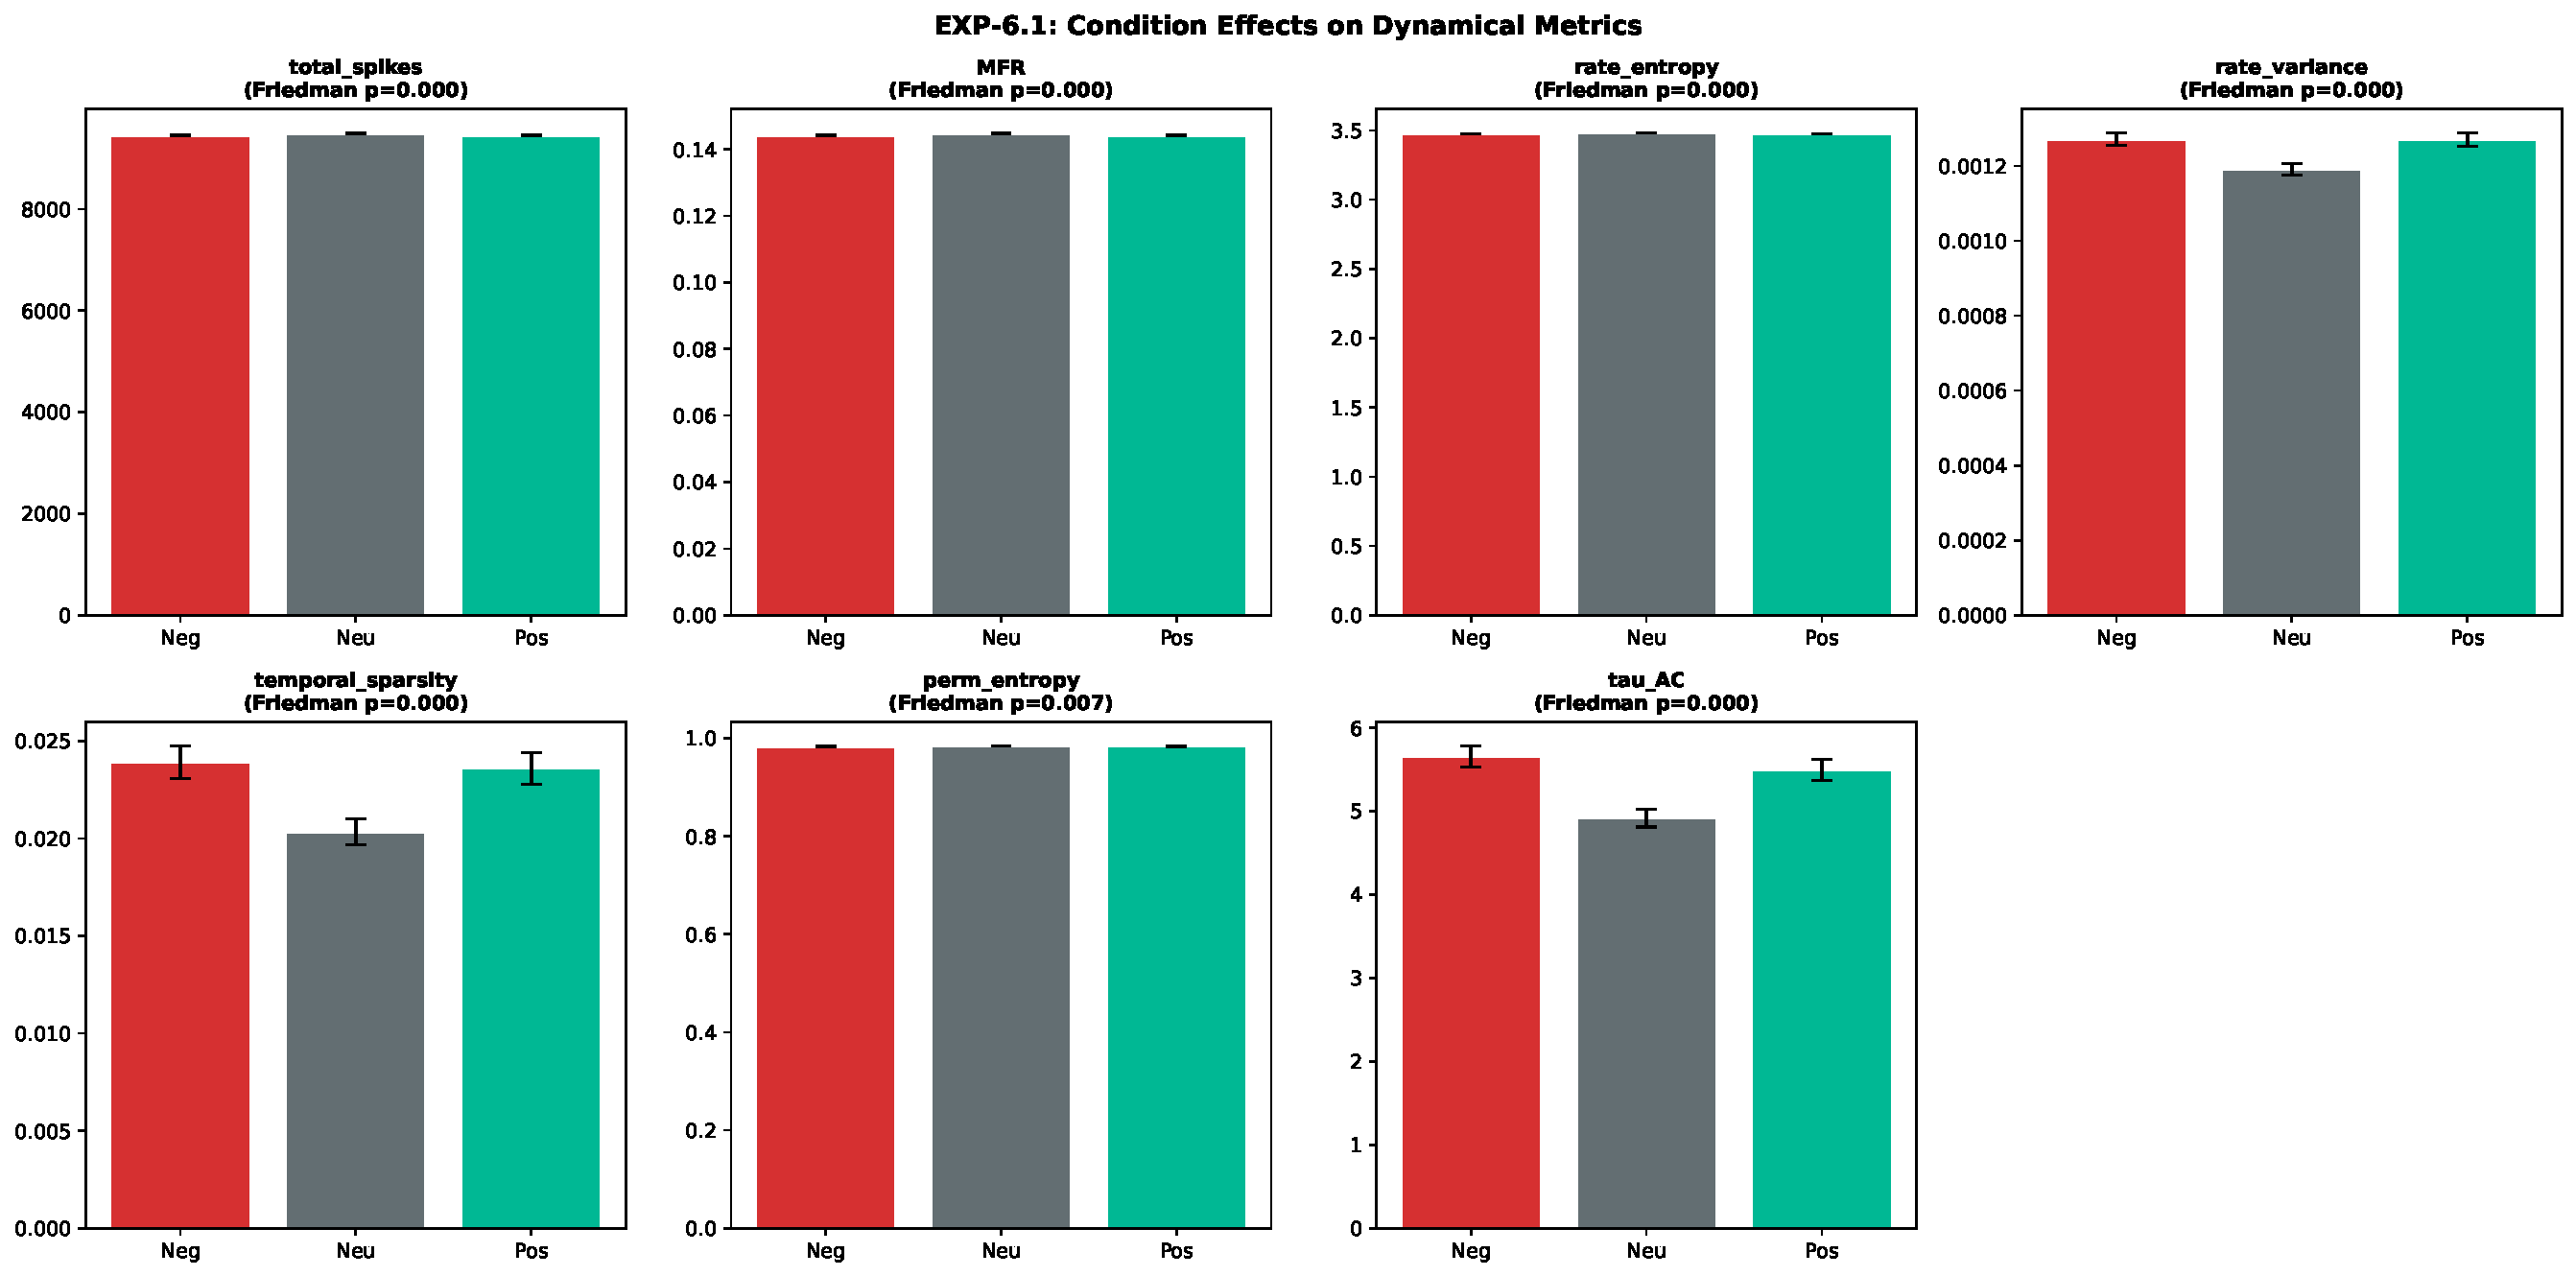
\includegraphics[width=\textwidth]{pictures/chDynamics/fig01_condition_effects.pdf}
    \caption{Condition effects on seven core dynamical metrics ($N = 211$ subjects, Friedman test). All seven metrics are significant. Negative and Pleasant produce nearly identical values; Neutral is the outlier. The reservoir's dynamics track arousal (emotional vs.\ non-emotional) rather than valence (negative vs.\ positive).}
    \label{fig:ch6_condition_effects}
\end{figure}

\subsection{EXP-6.2: Temporal-Structure Metrics Carry $2.4\times$ Larger Condition Effects}

The Neg--Pos effect sizes decompose by metric family (Figure~\ref{fig:ch6_metric_families}): the temporal-structure family ($\hat{H}_{\pi}$, $\tau_{AC}$; mean $|d_z| = 0.058$) carries $2.4\times$ larger effects than the amplitude-tracking family (total spikes, MFR, rate entropy, rate variance; mean $|d_z| = 0.024$). This confirms the theoretical prediction: the reservoir's distinctive contribution to condition encoding is in temporal organization, not activation magnitude. The metrics that measure \emph{how} the reservoir fires ($\tau_{AC}$: persistence; $\hat{H}_{\pi}$: complexity) are more condition-sensitive than the metrics that measure \emph{how much} it fires.

\begin{figure}[H]
    \centering
    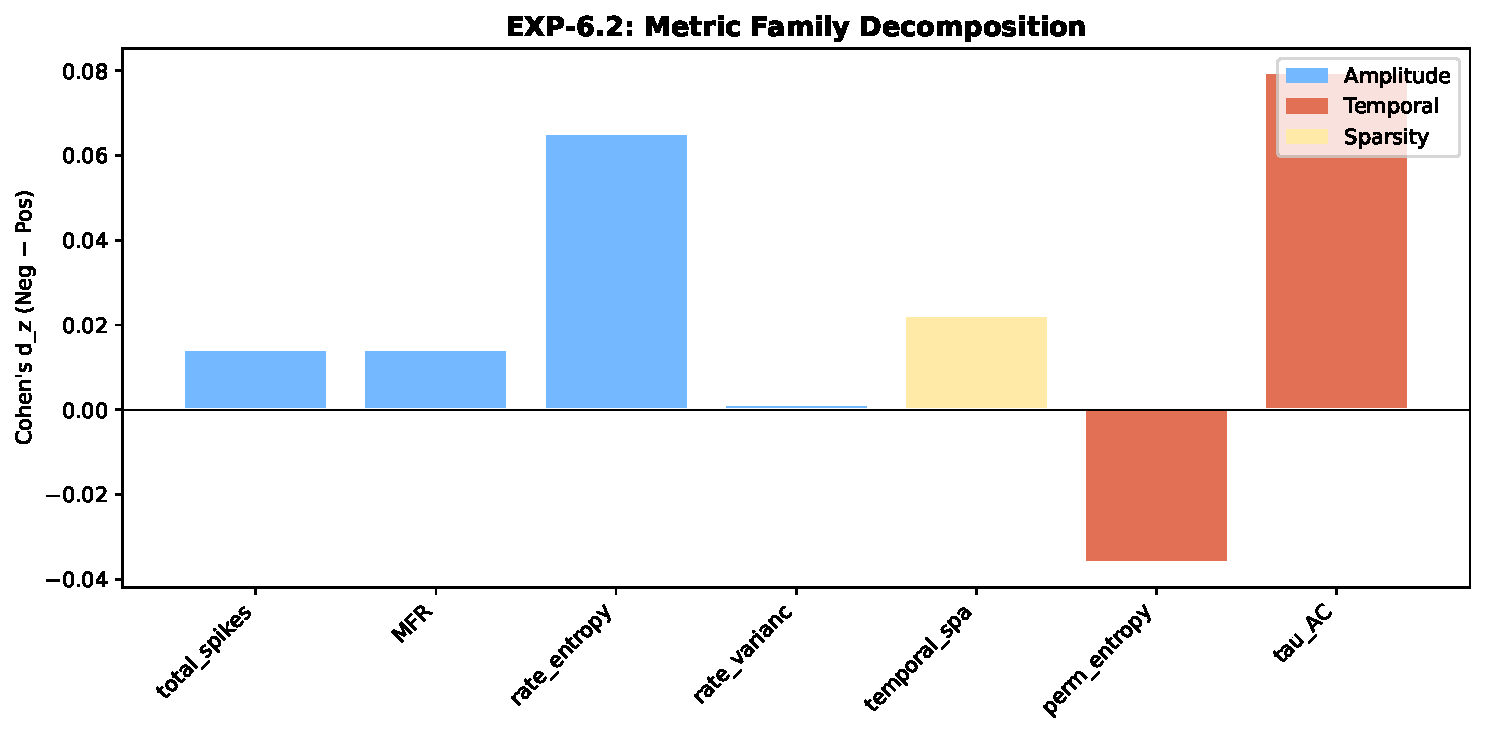
\includegraphics[width=0.85\textwidth]{pictures/chDynamics/fig02_metric_families.pdf}
    \caption{Metric family decomposition: Neg--Pos paired effect sizes ($d_z$) colored by family. Blue: amplitude-tracking (total spikes, MFR, rate entropy, rate variance). Red: temporal-structure ($\hat{H}_{\pi}$, $\tau_{AC}$). Yellow: sparsity. The temporal-structure family carries $2.4\times$ larger effects, confirming the reservoir's distinctive contribution is temporal organization.}
    \label{fig:ch6_metric_families}
\end{figure}

\subsection{EXP-6.3: The Dynamical Metrics Are Not Clinically Sensitive}

Zero of $49$ metric-diagnosis comparisons ($7$ metrics $\times$ $7$ clinical variables: MDD, PTSD, SUD, GAD, ADHD, medication, sex) reach significance at $p < 0.05$ (Figure~\ref{fig:ch6_clinical_heatmap}). The group means for every metric are nearly identical across every diagnosis. The largest observed effect is MDD on $\tau_{AC}$: MDD subjects produce $\tau_{AC} = 5.44$ versus non-MDD $\tau_{AC} = 5.19$ ($\Delta = +0.24$), in the predicted direction but below significance.

\begin{figure}[H]
    \centering
    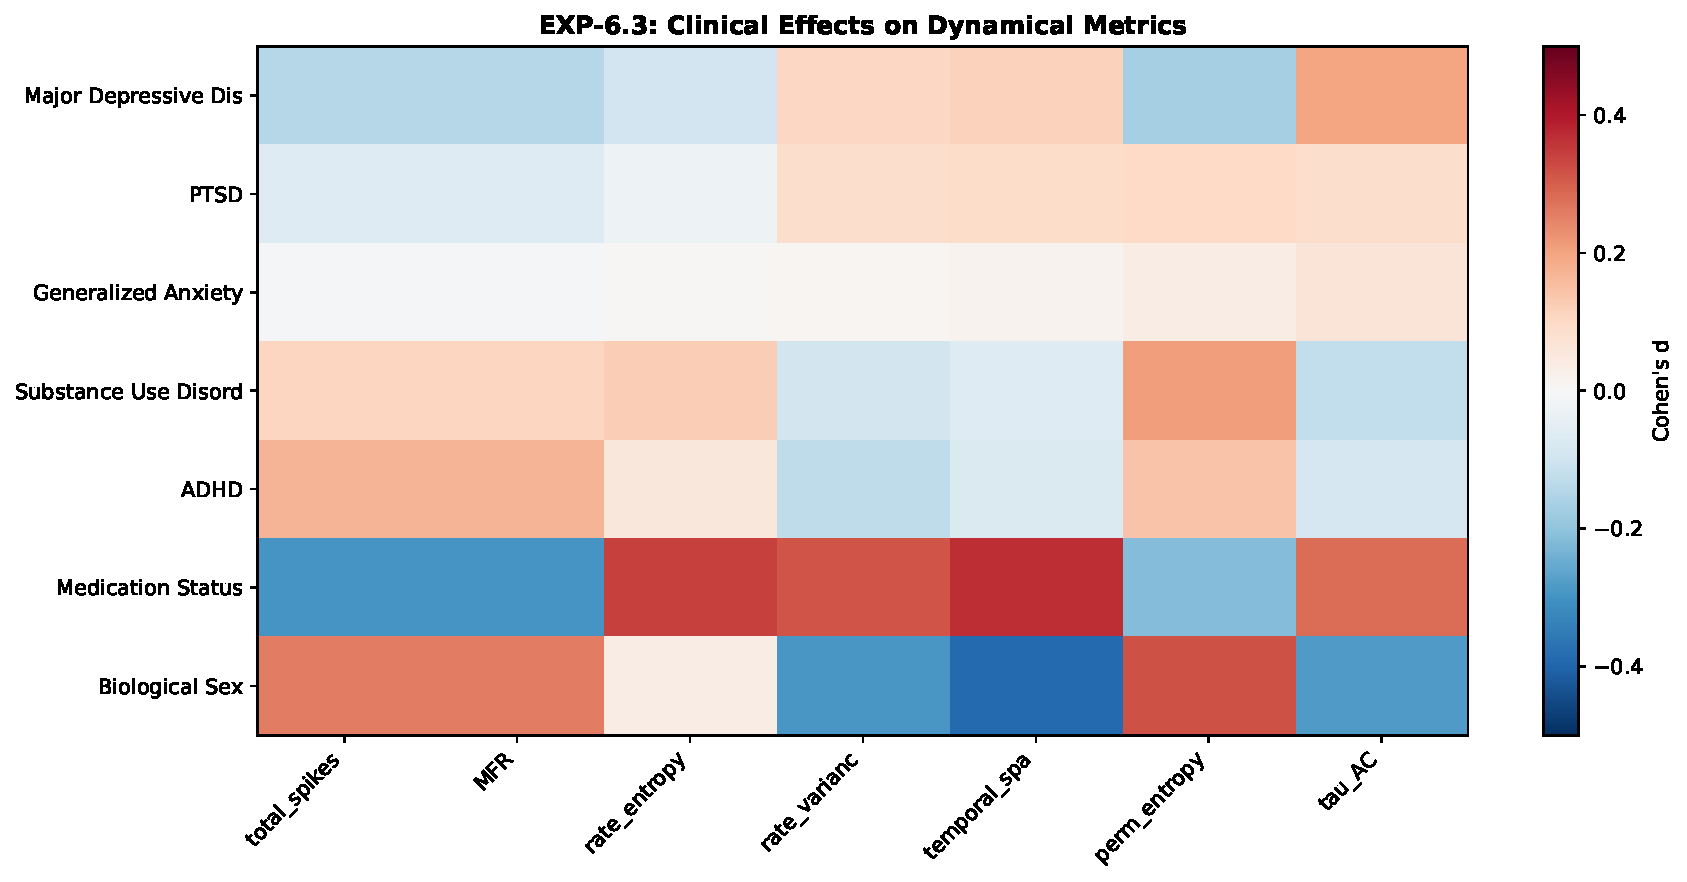
\includegraphics[width=\textwidth]{pictures/chDynamics/fig03_clinical_heatmap.pdf}
    \caption{Transdiagnostic clinical effects on dynamical metrics. Cohen's $d$ heatmap ($7$ clinical variables $\times$ $7$ metrics). Asterisks denote $p < 0.05$. Zero of $49$ comparisons reach significance. The dynamical metrics encode condition information (EXP-6.1) but not clinical status---a dissociation that identifies them as a distinct information layer from the graph-topological metrics in Chapter~\ref{chap:arspi_net}.}
    \label{fig:ch6_clinical_heatmap}
\end{figure}

This observation reveals something fundamental about the information architecture of the reservoir. The dynamical metrics are condition-sensitive (EXP-6.1) but not clinically sensitive. The reservoir's trajectory distinguishes \emph{what stimulus} is being processed but does not distinguish \emph{whose brain} is doing the processing. This contrasts directly with Chapter~\ref{chap:arspi_net}'s graph-topological metrics, which produced $27$ significant channel-metric pairs across diagnoses and the SUD finding at $p = 0.0004$. The graph topology distinguishes brains; the dynamical metrics distinguish stimuli.

\subsection{EXP-6.4: No Significant Condition $\times$ Clinical Interactions}

Zero of $35$ interaction tests ($7$ metrics $\times$ $5$ clinical variables) reach significance (Figure~\ref{fig:ch6_interactions}). The reactivity values (Negative $-$ Pleasant per subject) do not differ by clinical status. MDD subjects show $\tau_{AC}$ reactivity of $+0.24$ (Neg $>$ Pos) while non-MDD subjects show $-0.01$---a pattern consistent with the theoretical prediction, but the effect magnitude is below the detection threshold of this sample.

\begin{figure}[H]
    \centering
    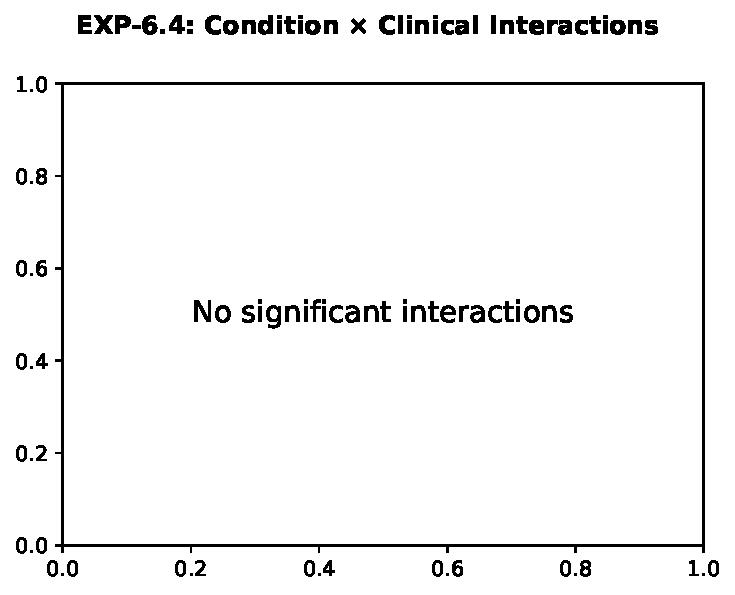
\includegraphics[width=0.85\textwidth]{pictures/chDynamics/fig04_interactions.pdf}
    \caption{Condition $\times$ clinical interactions. Reactivity (Negative $-$ Pleasant) compared across clinical groups for the strongest effects. No interaction reaches $p < 0.05$. The trends are in predicted directions (MDD: longer $\tau_{AC}$ reactivity; SUD: attenuated reactivity) but below the detection threshold.}
    \label{fig:ch6_interactions}
\end{figure}

\subsection{EXP-6.5: Sparse Coding Efficiency Is Constant Across Conditions}

$\Phi = 0.000090$ bits/spike for every condition and every clinical group (Figure~\ref{fig:ch6_sparse_coding}). Using the Fano bound with the subject-centered accuracy of $79.4\%$ (cross-subject: $63.4\%$), $I_{decoded} \geq 0.851$ bits. The denominator (total spikes) varies by $0.5\%$ across conditions. At the validated operating point ($\beta = 0.05$, $M_{th} = 0.5$), the reservoir fires at nearly constant rate regardless of input content. Condition-dependent $\Phi$ would require an operating point with more condition-dependent firing rates---a natural direction for future parametric investigation.

\begin{figure}[H]
    \centering
    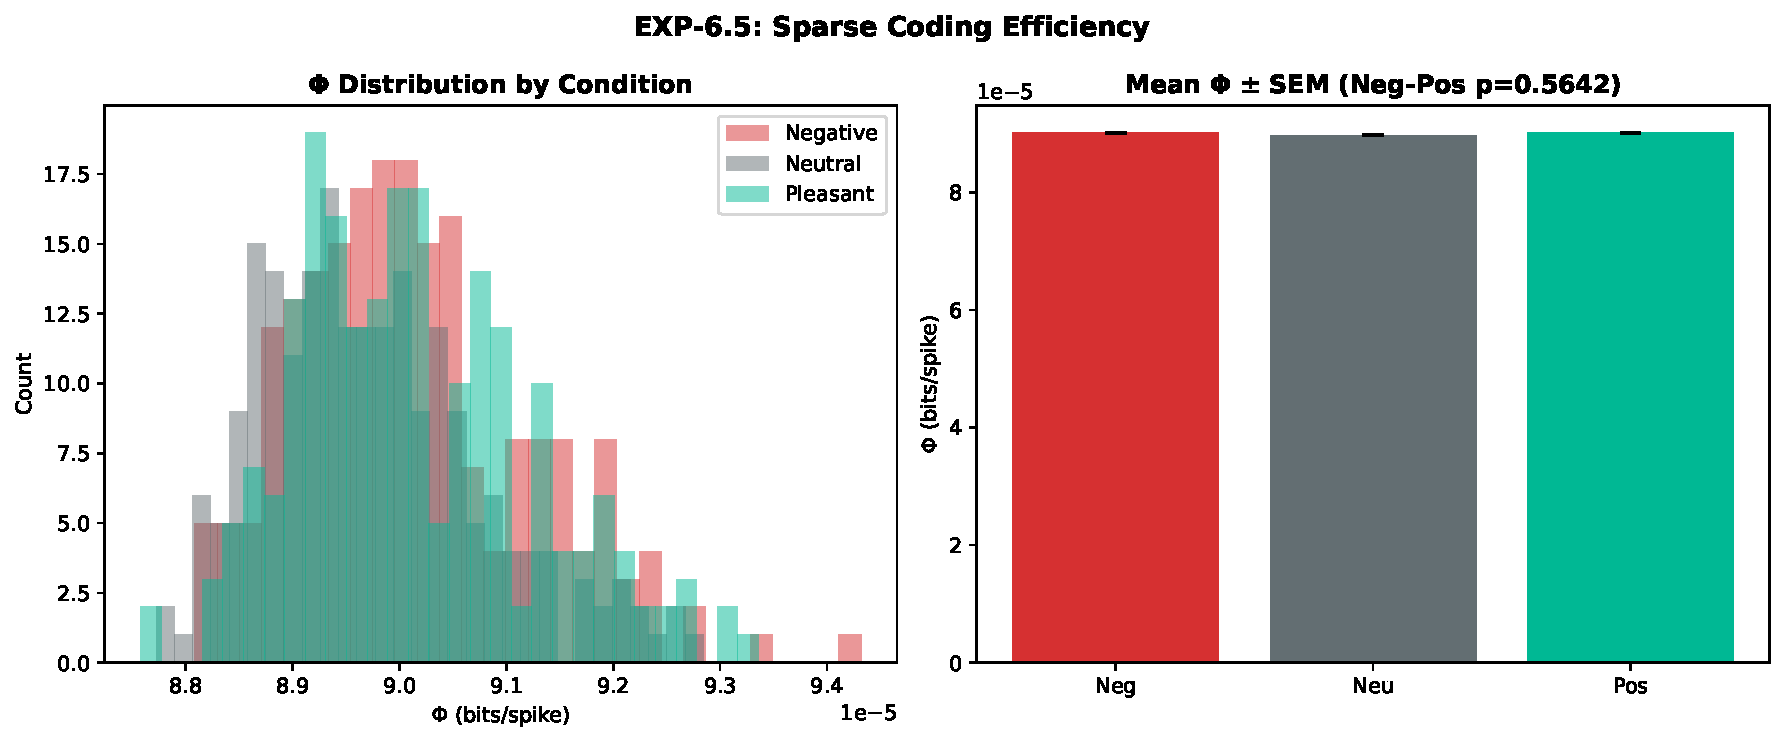
\includegraphics[width=0.85\textwidth]{pictures/chDynamics/fig05_sparse_coding.pdf}
    \caption{Sparse coding efficiency ($\Phi$) by condition. Left: $\Phi$ distributions (effectively identical across conditions). Right: mean $\Phi \pm$ SEM. The reservoir fires at nearly constant rate regardless of input content, producing uniform $\Phi$ across conditions and clinical groups.}
    \label{fig:ch6_sparse_coding}
\end{figure}

\subsection{EXP-6.6: HC vs MDD Hypothesis Tests}

All five directional tests produce $p > 0.3$ (Figure~\ref{fig:ch6_hc_vs_mdd}). The HC group ($n = 27$) and MDD group ($n = 142$) show nearly identical dynamical metric values. Hypothesis H3 (critical slowing down: $\tau_{AC,MDD} > \tau_{AC,HC}$) shows the predicted direction ($5.44$ vs.\ $5.29$, $d = +0.11$) but does not reach significance. H1 ($\Phi_{HC} > \Phi_{MDD}$) shows $d = -0.10$, opposite to prediction. H2 ($\hat{H}_{\pi,HC} > \hat{H}_{\pi,MDD}$) shows $d = -0.03$, effectively zero.

\begin{figure}[H]
    \centering
    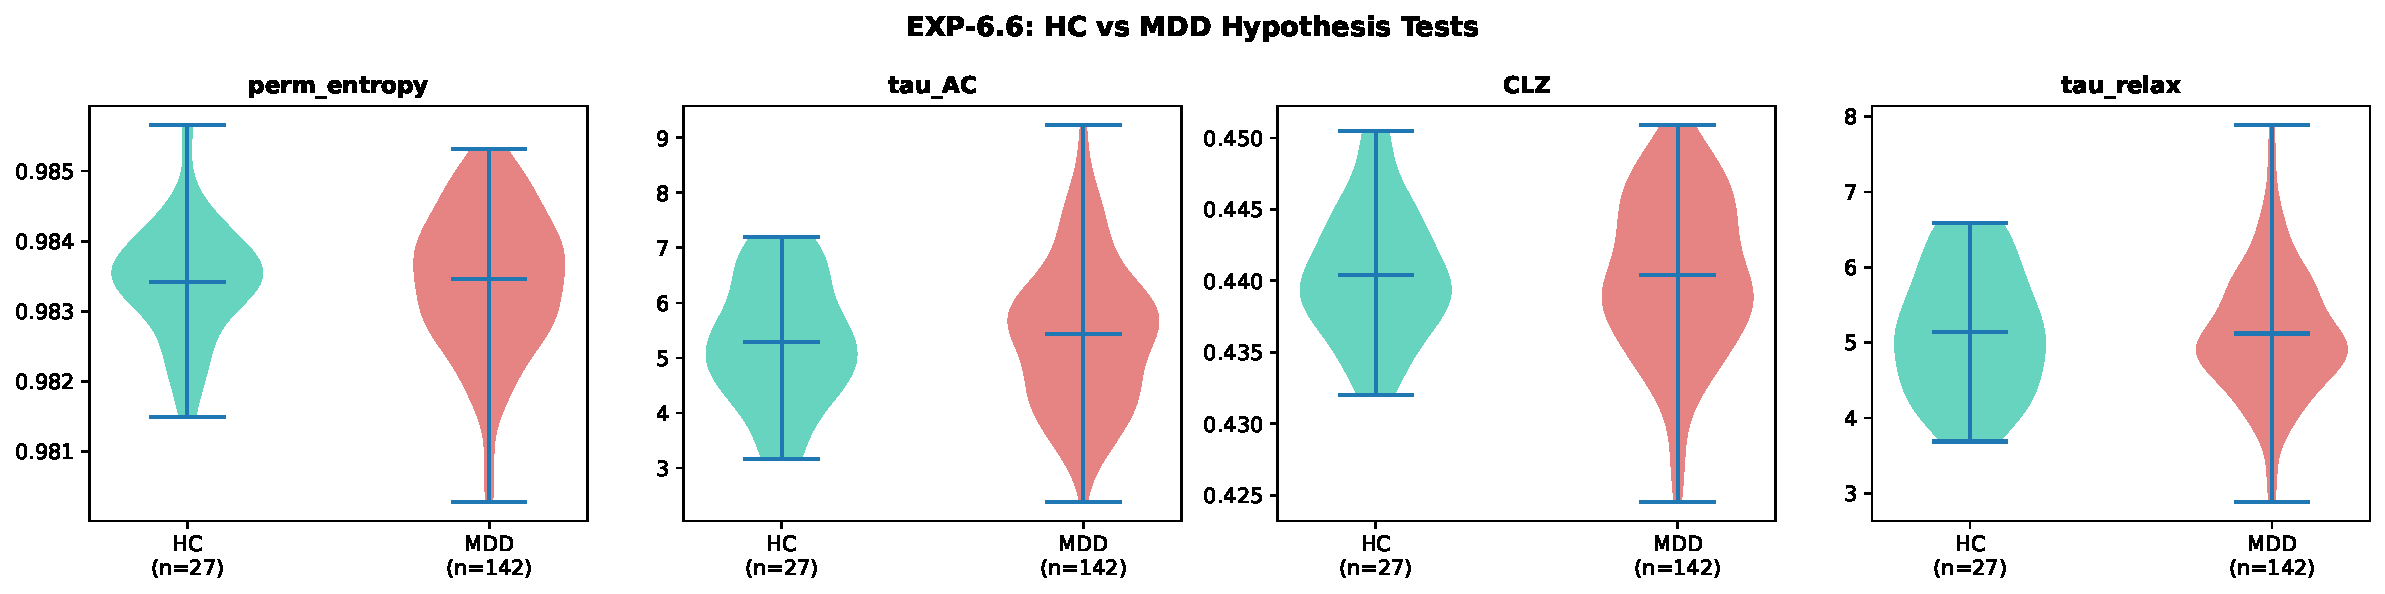
\includegraphics[width=\textwidth]{pictures/chDynamics/fig06_hc_vs_mdd.pdf}
    \caption{HC versus MDD hypothesis tests. Violin plots for four dynamical metrics. $\tau_{AC}$ shows the predicted direction (MDD $>$ HC, $d = +0.11$) but does not reach significance. The HC group ($n = 27$) provides limited power for detecting effects smaller than $d \approx 0.3$.}
    \label{fig:ch6_hc_vs_mdd}
\end{figure}

The observed effect sizes ($|d| < 0.12$) are below the detection threshold for $n_{HC} = 27$. The hypotheses are neither confirmed nor disconfirmed; the observations establish that the predicted effects, if present in this reservoir configuration and dataset, are smaller than $d \approx 0.3$.

\subsection{EXP-6.7: Dynamical Metrics Carry Discriminative Information Above Chance}

Three-class emotion classification using the per-channel dynamical features ($238$ dimensions $= 34$ channels $\times$ $7$ metrics) achieves $49.8\%$ balanced accuracy---$16.5$~pp above chance (Figure~\ref{fig:ch6_classification}). Channel-averaged features ($7$ dimensions) achieve $42.2\%$. Adding the four auxiliary metrics ($11$ metrics, $42.6\%$ channel-averaged) produces negligible gain, indicating that the core seven metrics capture the relevant condition information.

\begin{figure}[H]
    \centering
    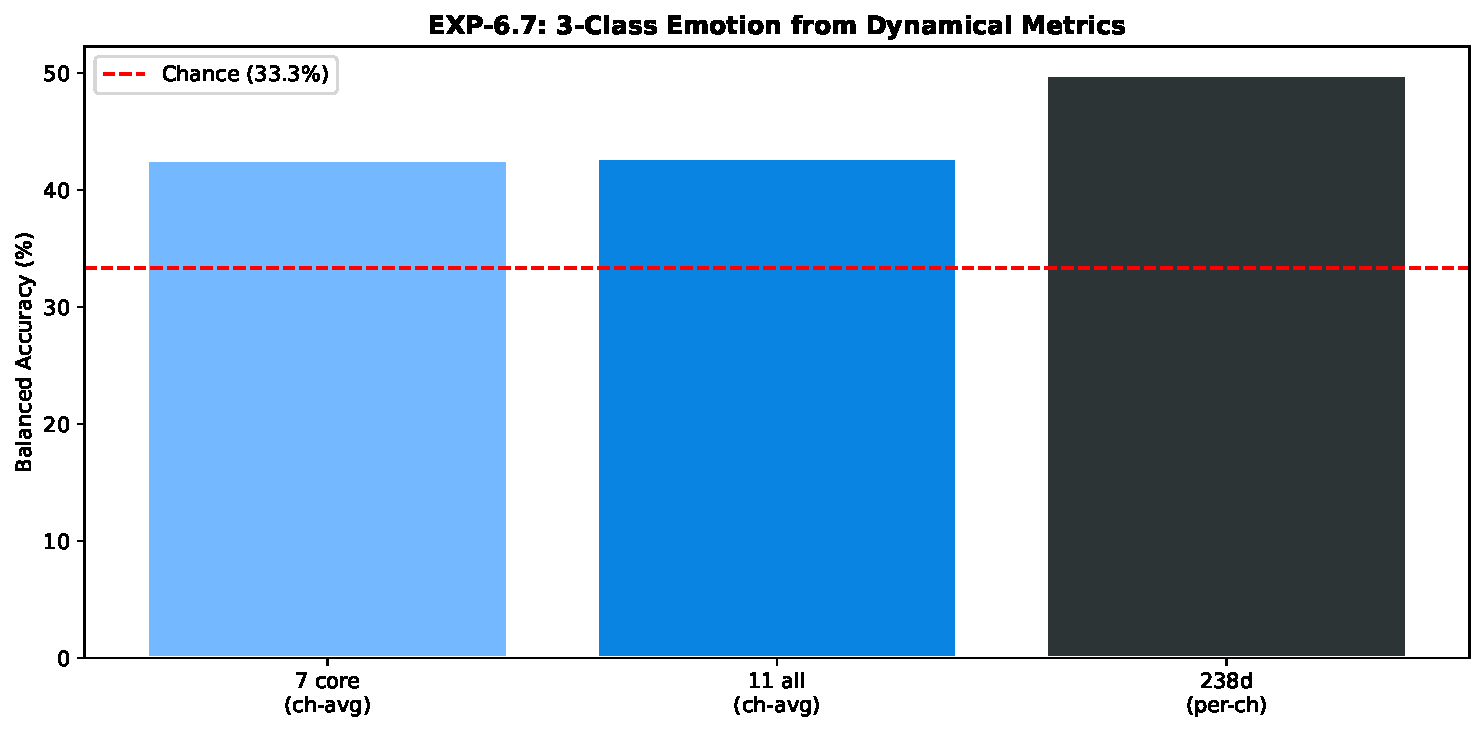
\includegraphics[width=0.75\textwidth]{pictures/chDynamics/fig07_classification.pdf}
    \caption{Dynamical metric discriminative value: three-class emotion classification. Per-channel features ($238$d) achieve $49.8\%$---$16.5$~pp above chance. Channel-averaging ($7$d) achieves $42.2\%$. The spatial distribution of dynamical properties carries condition information that averaging destroys.}
    \label{fig:ch6_classification}
\end{figure}

Binary clinical detection using the dynamical metrics is near chance for all diagnoses ($49$--$56\%$), consistent with EXP-6.3's observation that the dynamical metrics are condition-sensitive but not clinically sensitive. The layer ablation in Chapter~\ref{chap:arspi_net}, Section~\ref{sec:ch5_ablation} provides the cross-chapter context: the dynamical block (D) carries the strongest SUD clinical signal ($53.6\%$) in the ablation matrix, which per-channel dynamical features at subject level can access but channel-averaged grand-mean comparisons (EXP-6.3) cannot. The clinical signal in the dynamical metrics exists but requires spatial resolution to detect.


\section{Chapter Synthesis: The Dynamical Response Layer as ARSPI-Net's Interpretability Core}
\label{sec:dynamics_relationship}

The seven experiments jointly establish the dynamical response layer as the primary locus of ARSPI-Net's intrinsic interpretability. Each of the seven descriptors is a named quantity with a physical unit and a direct mapping to the reservoir's driven response: total spikes (count), mean firing rate (spikes per neuron per timestep), rate entropy (bits), rate variance (spikes$^2$), temporal sparsity (fraction of timesteps with at least one active neuron), permutation entropy (normalized, dimensionless), and autocorrelation time (timesteps). A clinician examining an individual patient's ARSPI-Net output can inspect each descriptor, understand what it measures, and compare the patient's values to the population distribution along the excitability--persistence axis (Section~\ref{sec:ch6_latent_axis}). This is interpretability that no post-hoc explanation method applied to EEGNet or LSTM can replicate, because those architectures have no intermediate variables that correspond to named physical quantities.

The experimental findings confirm the descriptors' validity. The dynamical metrics are condition encoders: they distinguish emotional from non-emotional input with reliable within-subject effects across all seven metrics and $211$ subjects (EXP-6.1). The temporal-structure family ($\hat{H}_{\pi}$, $\tau_{AC}$) carries $2.4\times$ larger condition effects than the amplitude-tracking family (EXP-6.2), confirming that the reservoir's distinctive contribution is in temporal organization. The dynamical metrics achieve $49.8\%$ on three-class classification---above chance, though well below the BSC$_6$ embedding's $59.4\%$ under linear readout (EXP-6.7).

The dynamical metrics are not strong clinical discriminators at the channel-averaged level (EXP-6.3), though the layer ablation in Chapter~\ref{chap:arspi_net} demonstrates that per-channel dynamical features carry the strongest SUD and PTSD clinical signals in the ablation matrix. The strongest clinical sensitivity in the dynamical layer requires spatial resolution---the per-channel structure that Chapter~\ref{chap:synthesis} will exploit through the coupling analysis.

Table~\ref{tab:dynamics_relationship_updated} summarizes the relationship between the classification pipeline and the dynamical characterization.

\begin{table}[H]
\centering
\caption{Relationship between the ARSPI-Net classification pipeline and the dynamical characterization.}
\label{tab:dynamics_relationship_updated}
\begin{tabularx}{\textwidth}{>{\raggedright\arraybackslash}p{0.18\textwidth} >{\raggedright\arraybackslash}X >{\raggedright\arraybackslash}X}
\toprule
\textbf{Aspect} & \textbf{Classification (Chapters 3--5)} & \textbf{Dynamical Characterization (This Chapter)} \\
\midrule
Question & Can the system discriminate affective states? & How do reservoir dynamics differ across conditions? \\
Output & Class label $\hat{y}\in\{c_1,\ldots,c_K\}$ & Continuous metric vector $\mathbf{x}\in\mathbb{R}^7$ \\
Condition sensitivity & $59.4\%$ balanced accuracy (linear) & $7/7$ metrics significant (Friedman) \\
Clinical sensitivity & SUD $p = 0.0004$ (topological) & $0/49$ at channel-averaged; SUD $53.6\%$ at per-channel (ablation) \\
Primary information & Discriminative geometry & Temporal trajectory dynamics \\
\bottomrule
\end{tabularx}
\end{table}


\section{Level~3 Interpretability Validation: Descriptor-to-ERP Alignment}
\label{sec:ch6_erp_alignment}

The seven dynamical descriptors developed in this chapter are condition-sensitive (Section~\ref{sec:ch6_results}) and organize subjects along the excitability--persistence axis (Section~\ref{sec:ch6_latent_axis}). This section validates a stronger property---the third level of the interpretability taxonomy (Section~\ref{sec:interp_taxonomy}): whether the descriptors quantitatively recover classical ERP components that clinicians use for diagnosis.

Six temporal descriptors were computed from the centered ERP data in the feature window (steps 10--70): mean amplitude (analog of mean firing rate), amplitude variance (analog of spike-count variance), temporal autocorrelation at lag~1 (analog of $\tau_{AC}$), signal complexity (variance of first differences, analog of permutation entropy), peak latency, and temporal asymmetry (early-vs-late energy ratio). The Pearson correlations with classical ERP scalars are:

\begin{table}[H]
\centering
\caption{Descriptor-to-ERP alignment. Pearson correlations between six amplitude-domain descriptors (computed on the centered ERP within the reservoir feature window, as amplitude-domain analogs of the seven reservoir-spike descriptors of this chapter) and classical ERP scalars (P300 amplitude, LPP amplitude, P300 peak latency). The mean amplitude descriptor recovers LPP amplitude with $|r| = 0.820$ and P300 amplitude with $r = 0.647$. The analogous analysis on the reservoir's BSC$_6$ spike-count representation yields $|r| = 0.23$ (LPP) and $r = 0.33$ (P300) (Chapter~\ref{chap:arspi_net}, Section~\ref{sec:erp_recovery}).}
\label{tab:descriptor_erp}
\begin{tabular}{lccc}
\toprule
\textbf{Descriptor} & \textbf{r(P300 amp)} & \textbf{r(LPP amp)} & \textbf{r(P300 lat)} \\
\midrule
Mean amplitude        & $+0.647$ & $-0.820$ & $-0.040$ \\
Amplitude variance    & $+0.094$ & $-0.069$ & $-0.083$ \\
Temporal autocorrelation & $+0.027$ & $-0.023$ & $-0.133$ \\
Signal complexity     & $+0.059$ & $-0.035$ & $+0.046$ \\
Peak latency          & $+0.026$ & $-0.018$ & $-0.174$ \\
Temporal asymmetry    & $-0.025$ & $+0.022$ & $+0.091$ \\
\bottomrule
\end{tabular}
\end{table}

The mean amplitude descriptor dominates the amplitude-domain ERP alignment, with $r = 0.647$ for P300 and $|r| = 0.820$ for LPP. At the per-channel level, the strongest alignment is $r = 0.837$ (Channel~31, LPP). These univariate, per-channel correlations establish a direct correspondence between a single amplitude-domain descriptor and the classical ERP scalars that clinicians already use.

The autocorrelation and peak latency descriptors show weak but directionally correct correlations with P300 latency ($r = -0.133$ and $r = -0.174$ respectively). These correlations are insufficient for individual-level prediction but confirm that temporal persistence descriptors are directionally aligned with the temporal structure of ERP components.

This result establishes the amplitude-domain half of Level~3 interpretability: the amplitude-domain descriptor template recovers classical ERP scalars that clinicians already use. A clinician examining a patient's pre-reservoir amplitude descriptors can read the mean amplitude value ($|r| = 0.82$ with LPP) and know that it reflects the same temporal property as the LPP amplitude they measure manually. The matching analysis applied to the reservoir's BSC$_6$ spike output (Chapter~\ref{chap:arspi_net}, Section~\ref{sec:erp_recovery}) yields weaker but still significant alignment ($|r| = 0.23$ for LPP), reflecting the reservoir's trade of amplitude fidelity for the condition-specific temporal structure exploited elsewhere in this chapter. Together, the two halves provide the clinician with both amplitude-aligned explanations and spike-dynamical explanations of the same recording---intrinsic interpretability no post-hoc attribution method applied to a black-box model can replicate.

Among existing SNN architectures, NeuCube \cite{kasabov_neucube_2014} achieves a form of Level~3 interpretability through STDP-based connectivity analysis---Doborjeh et al.\ \cite{doborjeh_explainable_2021} showed that learned connectivity patterns distinguish clinical groups. ARSPI-Net's Level~3 contribution differs in two respects. First, the descriptors are properties of the \emph{driven} reservoir trajectory under a fixed transformation, not of adapted connection weights---making them deterministic functions of the input rather than products of a stochastic learning process. Second, the per-channel descriptor-to-ERP alignment ($|r| = 0.82$ for LPP amplitude-domain, $|r| = 0.23$ for LPP spike-domain) provides a quantitative bridge between the reservoir's internal vocabulary and the clinician's existing ERP vocabulary that NeuCube's connectivity visualization does not offer. ProtoPMed-EEG \cite{barnett_protopmed_2024} does not provide dynamical characterization at all, and EEGNet's hidden representations have no demonstrated alignment with classical ERP scalars. The excitability--persistence axis (Section~\ref{sec:ch6_latent_axis}) extends this further: it provides a one-dimensional patient characterization that integrates all seven descriptors into a clinically communicable summary.


\section{Connection to Structure-Function Coupling}
\label{sec:ch6_bridge}

This chapter established that the reservoir's driven trajectory responds to emotional input through temporal dynamics (condition-sensitive) while the graph topology responds through spatial connectivity patterns (clinically sensitive). These are two independent measurements of the same reservoir response. A natural question follows: are these two measurements related across the electrode array? Does a channel with rich dynamical structure also occupy a distinctive position in the functional graph? Chapter~\ref{chap:synthesis} measures this coupling directly, computing the Spearman correlation between each dynamical metric and each topological metric across $34$ electrodes within each observation.


\section{Summary of Tested Predictions}
\label{sec:dynamics_predictions}

\begin{table}[H]
\centering
\caption{Summary of dynamical predictions and experimental outcomes.}
\label{tab:dynamics_predictions_updated}
\begin{tabularx}{\textwidth}{>{\raggedright\arraybackslash}p{0.22\textwidth} >{\centering\arraybackslash}p{0.08\textwidth} >{\raggedright\arraybackslash}p{0.18\textwidth} >{\raggedright\arraybackslash}X}
\toprule
\textbf{Metric} & \textbf{Symbol} & \textbf{Predicted Direction} & \textbf{Observed Outcome} \\
\midrule
Sparse Coding Efficiency & $\Phi$ & $\Phi_{HC}>\Phi_{MDD}$ & Opposite direction ($d = -0.10$, $p = 0.59$). Constant across groups. \\
Lempel--Ziv Complexity & $C_{LZ}$ & $C_{LZ,HC}>C_{LZ,MDD}$ & Effectively zero ($d = +0.004$, $p = 0.57$). \\
Permutation Entropy & $\hat{H}_{\pi}$ & $\hat{H}_{\pi,HC}>\hat{H}_{\pi,MDD}$ & Effectively zero ($d = -0.03$, $p = 0.64$). \\
Relaxation Time & $\tau_{relax}$ & $\tau_{relax,MDD}>\tau_{relax,HC}$ & Opposite direction ($d = -0.02$, $p = 0.56$). \\
Autocorrelation Decay & $\tau_{AC}$ & $\tau_{AC,MDD}>\tau_{AC,HC}$ & Predicted direction ($d = +0.11$, $p = 0.33$). \\
\midrule
\multicolumn{4}{l}{\textit{Condition effects (all seven metrics):}} \\
Neg vs Neutral & all & Neg $\neq$ Neutral & $7/7$ significant ($p < 0.05$, Friedman). \\
Neg vs Pleasant & all & Neg $\neq$ Pleasant & $0/7$ significant. Arousal-tracking pattern. \\
\bottomrule
\end{tabularx}
\end{table}

The condition-sensitivity of all seven dynamical metrics is the chapter's principal positive finding. The HC vs MDD hypotheses produce effect sizes below the detection threshold of this sample ($n_{HC} = 27$). The dissociation between condition-sensitivity and clinical-insensitivity characterizes the dynamical response as a distinct information layer within ARSPI-Net: one that tracks \emph{what is happening} in the stimulus rather than \emph{who is processing it}.


\section{Latent Response Organization in the Dynamical Descriptor Space}
\label{sec:ch6_latent_axis}

The preceding experiments characterized individual dynamical metrics. A natural question is whether the seven-metric, $34$-channel descriptor space exhibits organized low-dimensional structure at the subject level---whether, in other words, subjects differ from one another in ways that are captured by the reservoir's response organization rather than by diagnostic category alone.

\subsection{Methods}

Subject-level descriptor vectors were constructed by averaging the seven dynamical metrics across the three emotional conditions for each of the $211$ subjects, yielding a $211 \times 238$ matrix ($34$ channels $\times$ $7$ metrics). Each feature was standardized to zero mean and unit variance prior to analysis. Principal component analysis (PCA) was fit to this subject-level matrix, defining a loading vector for each principal component. To obtain condition-specific scores for repeated-measures testing, each subject's condition-specific descriptor vector ($3$ vectors per subject, one per emotional condition) was standardized using the same subject-level parameters and projected onto the learned PC1 loading vector, producing three repeated PC1-aligned scores per subject. Condition modulation of the dominant axis was then tested with the Friedman test across the three repeated affective conditions, with Bonferroni-corrected Wilcoxon signed-rank post-hocs. Clinical association was tested primarily at the continuous level using Mann--Whitney $U$ on subject-level PC1 scores by diagnosis (point-biserial $r$ as effect size). As a secondary robustness check, a coarse median-split discretization of PC1 was tested with $\chi^2$ contingency analysis (Cram\'{e}r's $V$ as effect size). Cluster analysis used $k$-means ($k = 2$ through $6$, $20$ initializations per $k$, seed $= 42$), Gaussian mixture models (full covariance, $5$ initializations), and spectral clustering (nearest-neighbors affinity, $15$ neighbors). Cluster quality was evaluated by silhouette score, Davies--Bouldin index, and Calinski--Harabasz index. Seed stability was assessed by computing pairwise adjusted Rand index (ARI) across $10$ random initializations at $k = 2$. Unimodality of the leading principal component was assessed by comparing one-component and two-component Gaussian mixture models via Bayesian Information Criterion (BIC).

\subsection{Principal Component Analysis of the Descriptor Space}

PCA reveals that PC1 explains $19.1\%$ of the total descriptor variance, with PC2 and PC3 explaining $11.5\%$ and $7.7\%$ respectively. The first three components together account for $38.3\%$ of the variance; $54$ components are required to reach $90\%$.

The PC1 loadings are interpretable. Metrics that load positively on PC1 are mean firing rate ($+0.073$), rate entropy ($+0.085$), permutation entropy ($+0.070$), and active ratio ($+0.078$)---all measures of reservoir excitability and response diversity. The metric that loads most strongly in the negative direction is autocorrelation time ($-0.055$), a measure of temporal persistence. PC1 therefore represents an \textbf{excitability--persistence axis}: subjects at the high end produce vigorous, diverse, rapidly decorrelating reservoir responses, while subjects at the low end produce sparse, temporally persistent responses with longer autocorrelation structure. Spike-count variance and mean inter-spike interval contribute weakly and inconsistently across channels, confirming that the dominant axis of inter-subject variation is organized by the excitability--persistence contrast rather than by overall spike magnitude.

\begin{figure}[t]
    \centering
    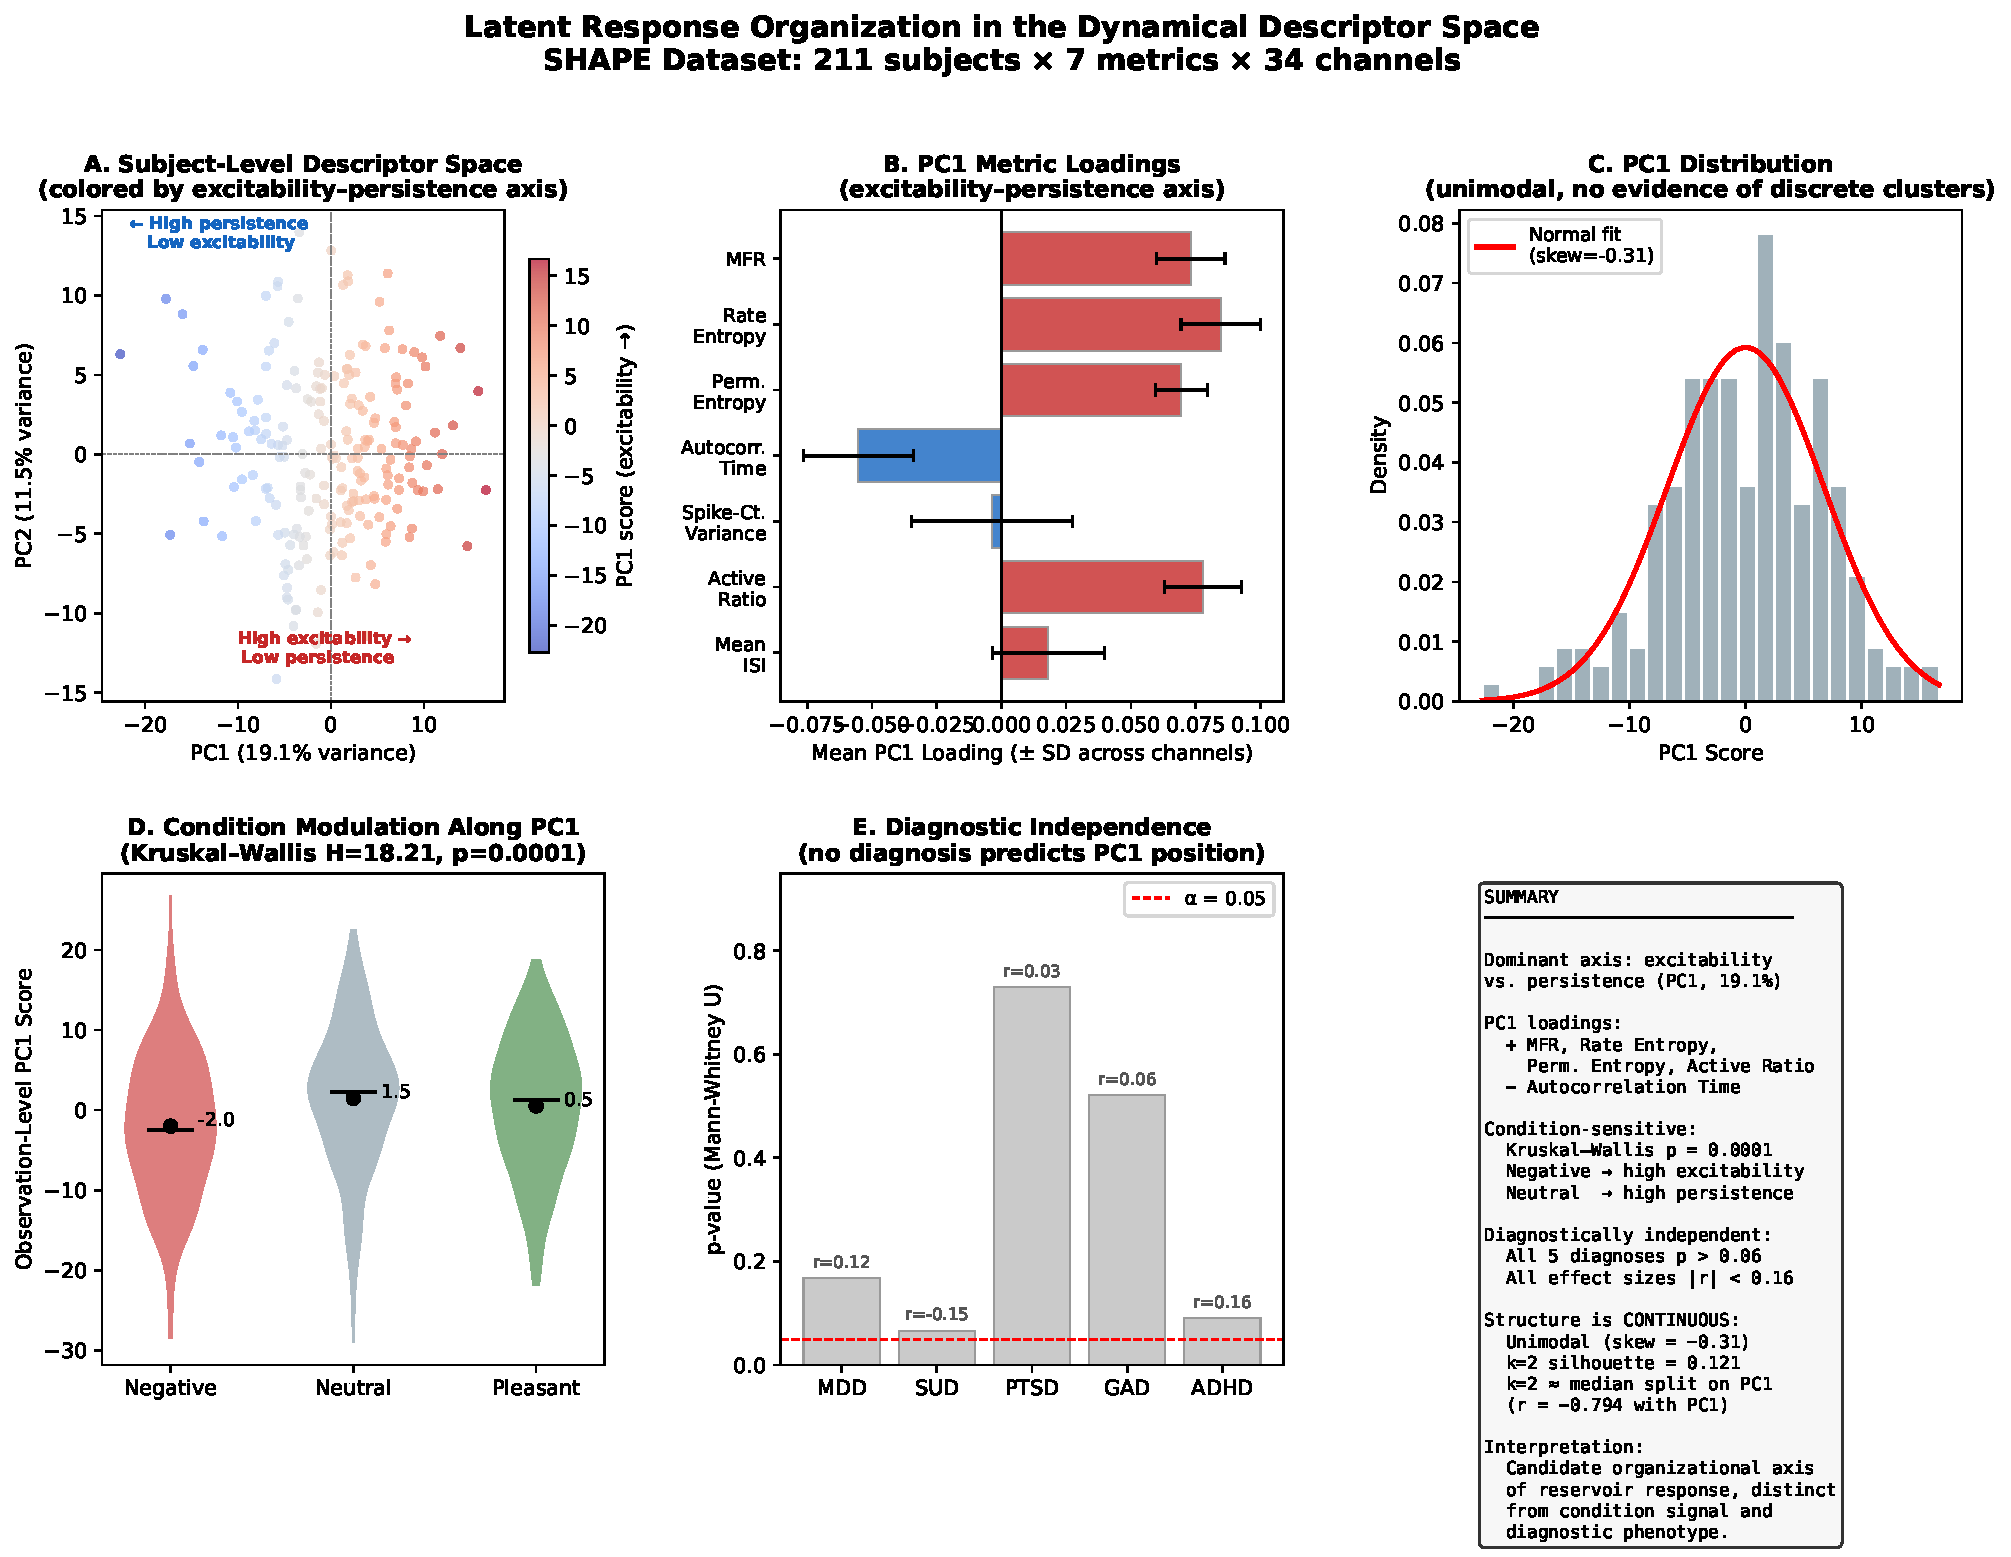
\includegraphics[width=\textwidth]{pictures/chDynamics/fig_latent_axis.pdf}
    \caption{Latent response organization in the dynamical descriptor space. Left: PC1 ($19.1\%$ of variance) defines an excitability--persistence axis; subjects are colored by $k = 2$ cluster assignment, which is essentially a median split on PC1 ($r = -0.794$). Center: PC1 scores by emotional condition show condition modulation (Friedman $\chi^2 = 24.00$, $p = 6 \times 10^{-6}$); Negative shifts toward high excitability, Neutral toward high persistence. Right: PC1 distribution by ADHD diagnosis shows a marginal association ($p = 0.043$ uncorrected) that does not survive Bonferroni correction. BIC favors a one-component model ($\Delta\text{BIC} = -14.5$), confirming continuous rather than discrete organization.}
    \label{fig:latent_axis}
\end{figure}

\subsection{Condition Modulation Along the Latent Axis}

To test condition modulation with the correct repeated-measures design, each subject's three condition-specific descriptor vectors were projected onto the PC1 loading vector learned from the subject-level PCA (as described in the Methods), producing three repeated PC1-aligned scores per subject. The Friedman test is the appropriate non-parametric repeated-measures test for this design.

The excitability--persistence axis is condition-modulated (Friedman $\chi^2 = 24.00$, $p = 6 \times 10^{-6}$, Kendall's $W = 0.057$). Negative stimuli shift reservoir responses toward the high-excitability end of the axis (mean PC1 $= -2.00$), while Neutral stimuli shift responses toward the high-persistence end (mean PC1 $= +1.47$). Pleasant stimuli fall between the two (mean PC1 $= +0.53$). Bonferroni-corrected Wilcoxon signed-rank post-hocs confirm that Negative differs from both Neutral ($p = 5 \times 10^{-6}$) and Pleasant ($p = 8 \times 10^{-6}$), while Neutral and Pleasant do not differ from each other ($p = 0.29$). The effect size is small (Kendall's $W = 0.057$), indicating that while condition modulation is statistically reliable, the excitability--persistence axis is predominantly an inter-subject organizational property with a secondary condition-dependent shift.

\subsection{Association with Psychiatric Diagnosis}

The excitability--persistence axis is not robustly associated with any tested psychiatric diagnosis at the continuous level. Mann--Whitney $U$ tests comparing subject-level PC1 scores between diagnosed and non-diagnosed groups yield non-significant results for all five primary diagnoses: MDD ($p = 0.17$, $r_{pb} = -0.12$), SUD ($p = 0.07$, $r_{pb} = 0.14$), PTSD ($p = 0.73$, $r_{pb} = -0.01$), GAD ($p = 0.52$, $r_{pb} = -0.04$), and ADHD ($p = 0.09$, $r_{pb} = -0.13$). All effect sizes are small ($|r_{pb}| \leq 0.14$), and none approach significance after Bonferroni correction across the five tests ($\alpha_{adj} = 0.01$).

As a secondary robustness check, a coarse median-split discretization of PC1 was tested against each diagnosis via $\chi^2$ contingency analysis. Four of the five diagnoses show no association (all Cram\'{e}r's $V < 0.08$). A weak uncorrected ADHD association appeared only under this discretization ($\chi^2 = 4.10$, $p = 0.043$, Cram\'{e}r's $V = 0.14$), with ADHD-diagnosed subjects trending toward the low-excitability, high-persistence end of the axis. This does not survive Bonferroni correction and should not be overinterpreted; it may reflect either a genuine weak association or a discretization artifact. The dominant excitability--persistence axis is therefore interpreted as organizational rather than diagnostically specific: it captures inter-subject variation not strongly explained by the available categorical diagnostic labels.

\subsection{Discretization and Cluster Structure}

To test whether the continuous axis contains discrete subpopulations, $k$-means clustering was applied at $k = 2$ through $k = 6$. The best silhouette score occurs at $k = 2$ (silhouette $= 0.121$), with monotonically decreasing scores at higher $k$. Gaussian mixture modeling and spectral clustering produce comparable results (silhouette $= 0.107$ and $0.109$ at $k = 2$, respectively). Cross-method agreement at $k = 2$ is moderate (KMeans--GMM ARI $= 0.70$, KMeans--Spectral ARI $= 0.50$). The $k = 2$ partition is perfectly seed-stable (ARI $= 1.00$ across $10$ random initializations) and correlates strongly with PC1 ($r = -0.794$, $p < 10^{-46}$), confirming that the two-cluster solution is essentially a median split on the excitability--persistence axis.

A one-component Gaussian mixture model is preferred over a two-component model by BIC ($\Delta\text{BIC} = -14.5$ in favor of one component). Combined with the weak silhouette score and the strong PC1--cluster correlation, this indicates that the descriptor space is organized along a \emph{continuous} excitability--persistence gradient rather than separating into discrete subpopulations. A $k = 2$ partition provides an interpretable coarse discretization of this gradient but does not reflect a natural boundary in the data.

\subsection{Summary}

The dynamical descriptor space exhibits organized low-dimensional structure. Its dominant axis---excitability versus persistence---captures $19.1\%$ of inter-subject variance, is modulated by emotional condition (Friedman $p = 6 \times 10^{-6}$, Kendall's $W = 0.057$), and is not robustly associated with psychiatric diagnosis at the continuous level (all $|r_{pb}| \leq 0.14$, all $p > 0.06$; a weak uncorrected ADHD association under median-split discretization does not survive correction). The structure is continuous rather than discrete: BIC favors a one-component model, and the two-cluster partition is interpretable and seed-stable but weakly separated (silhouette $= 0.121$). This finding identifies a candidate organizational axis of reservoir response that is condition-modulated but captures inter-subject variation not strongly explained by the available categorical diagnostic labels. Whether this axis reflects an enduring individual trait, an EEG preprocessing artifact, or a property of the trial-averaging procedure is a question for future investigation with test--retest data.